\mfpicnumber{1}

\opengraphsfile{TheUnitCircle}

\setcounter{footnote}{0}

\label{TheUnitCircle}

In Section \ref{circularmotion}, we introduced circular motion and derived a formula which describes the linear velocity of an object moving on a circular path at a constant angular velocity.  One of the goals of this section is describe the \textit{position} of such an object.  To that end, consider an angle $\theta$ in standard position and let $P$ denote the point where the terminal side of $\theta$ intersects the Unit Circle.  By associating the point $P$ with the angle $\theta$, we are assigning a \emph{position} on the Unit Circle to the angle $\theta$.  The $x$-coordinate of $P$ is called the \index{cosine ! of an angle} \textbf{cosine} of $\theta$, written $\cos(\theta)$, while the $y$-coordinate of $P$ is called the \index{sine ! of an angle} \textbf{sine} of $\theta$, written $\sin(\theta)$.\footnote{The etymology of the name `sine' is quite colorful, and the interested reader is invited to research it;  the `co' in `cosine' is explained in Section \ref{Identities}.}  The reader is encouraged to verify that these rules used to match an angle with its cosine and sine do, in fact, satisfy the definition of a function.  That is, for each angle $\theta$, there is only one associated value of $\cos(\theta)$ and only one associated value of $\sin(\theta)$.  

\smallskip

\begin{tabular}{cc}

\begin{mfpic}[20]{-5}{5}{-5}{5}
\axes
\tlabel(4.75,-0.5){\scriptsize $x$}
\tlabel(0.25,5){\scriptsize $y$}
\tlabel(3.1,-0.75){\scriptsize $1$}
\tlabel(0.25,3.1){\scriptsize $1$}
\xmarks{-3 step 3 until 3}
\ymarks{-3 step 3 until 3}
\point[3pt]{(0,0)}
\drawcolor[gray]{0.7}
\circle{(0,0),3}
\drawcolor[rgb]{0.33,0.33,0.33}
\arrow \polyline{(0,0), (2.5, 4.3301)}
\arrow \parafcn{5, 55, 5}{1.5*dir(t)}
\tlabel[cc](1.9, 1){$\theta$}
\end{mfpic} 

&

\hspace{.25in}

\begin{mfpic}[20]{-5}{5}{-5}{5}
\axes
\tlabel(4.75,-0.5){\scriptsize $x$}
\tlabel(0.25,5){\scriptsize $y$}
\tlabel(3.1,-0.75){\scriptsize $1$}
\tlabel(0.25,3.1){\scriptsize $1$}
\xmarks{-3 step 3 until 3}
\ymarks{-3 step 3 until 3}
\arrow \polyline{(0,0), (2.5, 4.3301)}
\tlabel(2,2.6){$P(\cos(\theta), \sin(\theta))$}
\drawcolor[gray]{0.7}
\circle{(0,0),3}
\drawcolor[rgb]{0.33,0.33,0.33}
\arrow \parafcn{5, 55, 5}{1.5*dir(t)}
\tlabel[cc](1.9, 1){$\theta$}
\point[3pt]{(0,0), (1.5, 2.5981)}
\end{mfpic} 

\end{tabular}

%\smallskip

\begin{ex} \label{cosinesineviaunitcircle}  Find the cosine and sine of the following angles.

\begin{multicols}{5}

\begin{enumerate}

\item  $\theta = 270^{\circ}$

\item $\theta = - \pi$

\item  $\theta = 45^{\circ}$

\item  $\theta = \frac{\pi}{6}$

\item  $\theta = 60^{\circ}$

\end{enumerate}

\end{multicols}

{\bf Solution.}

\begin{enumerate}

\item  To find $\cos\left(270^{\circ}\right)$ and $\sin\left(270^{\circ}\right)$, we plot the angle $\theta =270^{\circ}$ in standard position and find the point on the terminal side of $\theta$ which lies on the Unit Circle.  Since $270^{\circ}$ represents $\frac{3}{4}$ of a counter-clockwise revolution, the terminal side of $\theta$ lies along the negative $y$-axis.  Hence, the point we seek is $(0,-1)$ so that  $\cos\left(270^{\circ}\right) = 0$ and $\sin\left(270^{\circ}\right) = -1$.

\item  The angle $\theta=-\pi$ represents one half of a clockwise revolution so its terminal side lies on the negative $x$-axis.  The point on the Unit Circle that lies on the negative $x$-axis is $(-1,0)$ which means  $\cos(-\pi) = -1$ and $\sin(-\pi) = 0$.

\begin{tabular}{cc}

\begin{mfpic}[18]{-5}{5}{-5}{5}
\axes
\tlabel(4.75,-0.5){\scriptsize $x$}
\tlabel(0.25,5){\scriptsize $y$}
\tlabel(3.1,-0.75){\scriptsize $1$}
\tlabel(0.25,3.1){\scriptsize $1$}
\tcaption{Finding $\cos\left(270^{\circ}\right)$ and $\sin\left(270^{\circ}\right)$}
\xmarks{-3 step 3 until 3}
\ymarks{-3 step 3 until 3}
\tlabel(0.25,-3.75){$P(0, -1)$}
\drawcolor[gray]{0.7}
\circle{(0,0),3}
\drawcolor[rgb]{0.33,0.33,0.33}
\arrow \parafcn{5, 265, 5}{1.5*dir(t)}
\tlabel(-2, 1.75){\scriptsize $\theta = 270^{\circ}$}
\point[3pt]{(0,0), (0, -3)}
\end{mfpic} 

&

\hspace{0.25in}

\begin{mfpic}[18]{-5}{5}{-5}{5}
\axes
\tlabel(4.75,-0.5){\scriptsize $x$}
\tlabel(0.25,5){\scriptsize $y$}
\tlabel(3.1,-0.75){\scriptsize $1$}
\tlabel(0.25,3.1){\scriptsize $1$}
\tcaption{Finding $\cos\left(-\pi\right)$ and $\sin\left( -\pi \right)$}
\xmarks{-3 step 3 until 3}
\ymarks{-3 step 3 until 3}
\tlabel(-5.5,0.5){$P(-1, 0)$}
\drawcolor[gray]{0.7}
\circle{(0,0),3}
\drawcolor[rgb]{0.33,0.33,0.33}
\arrow \parafcn{-5, -175, -5}{1.5*dir(t)}
\tlabel[cc](1, -2){\scriptsize $\theta=-\pi$}
\point[3pt]{(0,0), (-3, 0)}
\end{mfpic} 

\end{tabular}

\item  When we sketch $\theta = 45^{\circ}$ in standard position, we see that its terminal does not lie along any of the coordinate axes which makes our job of finding the cosine and sine values a bit more difficult. Let $P(x,y)$ denote the point on the terminal side of $\theta$ which lies on the Unit Circle. By definition,  $x = \cos\left(45^{\circ}\right)$ and $y = \sin\left(45^{\circ}\right)$.   If we drop a perpendicular line segment from $P$ to the $x$-axis, we obtain a $45^{\circ} - 45^{\circ} - 90^{\circ}$ right triangle whose legs have lengths $x$ and $y$ units. From Geometry,\footnote{Can you show this?} we get $y=x$.  Since $P(x,y)$ lies on the Unit Circle, we have $x^2+y^2 = 1$.  Substituting $y=x$ into this equation yields $2x^2 = 1$, or $x =\pm \sqrt{\frac{1}{2}} =  \pm \frac{\sqrt{2}}{2}$.  Since $P(x,y)$ lies in the first quadrant, $x>0$, so $x = \cos\left(45^{\circ}\right) = \frac{\sqrt{2}}{2}$ and with $y=x$ we have $y = \sin\left(45^{\circ}\right) = \frac{\sqrt{2}}{2}$.  

\medskip

\begin{tabular}{m{2.5in}m{1in}m{2.5in}}

\begin{mfpic}[18]{-5}{5}{-5}{5}
\axes
\tlabel(4.75,-0.5){\scriptsize $x$}
\tlabel(0.25,5){\scriptsize $y$}
\tlabel(4.1,-1){\scriptsize $1$}
\tlabel(0.25,4.1){\scriptsize $1$}
\xmarks{-4 step 4 until 4}
\ymarks{-4 step 4 until 4}
\tlabel(3.5,2.5){$P(x,y)$}
\drawcolor[gray]{0.7}
\circle{(0,0),4}
\drawcolor[rgb]{0.33,0.33,0.33}
\arrow \polyline{(0,0), (3.5355, 3.5355)}
\arrow \parafcn{5, 35, 5}{dir(t)}
\tlabel(1.15, .5){\scriptsize $\theta =  45^{\circ}$}
\point[3pt]{(0,0), (2.8284, 2.8284)}
\dashed \polyline{(2.8284, 2.8284), (2.8284, 0)}
\polyline{(2.5284, 0), (2.5284, 0.3), (2.8284, 0.3)}
\end{mfpic} 

&

&

\begin{mfpic}[18]{-5}{5}{-5}{5}
\polyline{(-2.5,0), (2.5,0), (2.5,5), (-2.5,0)}
\arrow \reverse \arrow \shiftpath{(-2.5,0)} \parafcn{5, 35, 5}{1.5*dir(t)}
\arrow \reverse \arrow \shiftpath{(2.5,5)}  \parafcn{230, 265, 5}{1.5*dir(t)}
\tlabel(-0.8, 0.4){$\theta =  45^{\circ}$}
\tlabel(1.4,2.8){$45^{\circ}$}
\tlabel(0,-0.5){$x$}
\tlabel(2.75,2.25){$y$}
\polyline{(2.25, 0), (2.25, 0.25), (2.5, 0.25)}
\point[3pt]{(2.5,5)}
\tlabel(2.75,5){$P(x,y)$}
\end{mfpic} 
\end{tabular}

\item  As before, the terminal side of $\theta = \frac{\pi}{6}$ does not lie on any of the coordinate axes, so we proceed using a triangle approach.  Letting $P(x,y)$ denote the point on the terminal side of $\theta$ which lies on the Unit Circle, we drop a perpendicular line segment from $P$ to the $x$-axis to form a $30^{\circ} - 60^{\circ} - 90^{\circ}$ right triangle.  After a bit of Geometry\footnote{Again, can you show this?} we find $y = \frac{1}{2}$ so $\sin\left(\frac{\pi}{6}\right) = \frac{1}{2}$.  Since $P(x,y)$ lies on the Unit Circle, we substitute $y = \frac{1}{2}$ into $x^2 + y^2 = 1$ to get $x^{2} = \frac{3}{4}$, or $x = \pm \frac{\sqrt{3}}{2}$.  Here, $x > 0$ so $x = \cos\left(\frac{\pi}{6}\right) = \frac{\sqrt{3}}{2}$.

\begin{tabular}{m{2.5in}m{0.5in}m{2.5in}}

\begin{mfpic}[18]{-5}{5}{-5}{5}
\axes
\tlabel(4.75,-0.5){\scriptsize $x$}
\tlabel(0.25,5){\scriptsize $y$}
\tlabel(4.1,-1){\scriptsize $1$}
\tlabel(0.25,4.1){\scriptsize $1$}
\xmarks{-4 step 4 until 4}
\ymarks{-4 step 4 until 4}
\tlabel(3.75,1.70){$P(x,y)$}
\drawcolor[gray]{0.7}
\circle{(0,0),4}
\drawcolor[rgb]{0.33,0.33,0.33}
\arrow \polyline{(0,0), (4.330,2.5)}
\arrow \parafcn{5, 25, 5}{1.5*dir(t)}
\tlabel(1.75, .25){\scriptsize $\theta =  \frac{\pi}{6}$}
\point[3pt]{(0,0), (3.4641, 2)}
\dashed \polyline{(3.4641,2), (3.4641, 0)}
\polyline{(3.1641, 0), (3.1641, 0.3), (3.4641, 0.3)}
\end{mfpic} 

&

&

\begin{mfpic}[18]{-5}{5}{-5}{5}
\polyline{(-4.330,0), (4.330,0), (4.330,5), (-4.330,0)}
\arrow \reverse \arrow \shiftpath{(-4.330,0)} \parafcn{5, 25, 5}{3*dir(t)}
\arrow \reverse \arrow \shiftpath{(4.330,5)}  \parafcn{215, 265, 5}{1.5*dir(t)}
\tlabel(-1, 0.6){$\theta = \frac{\pi}{6} = 30^{\circ}$}
\tlabel(2.75,2.9){$60^{\circ}$}
\tlabel(0,-0.75){$x$}
\tlabel(4.75,2.25){$y$}
\polyline{(3.93, 0), (3.93, 0.4), (4.33, 0.4)}
\point[3pt]{(4.330,5)}
\tlabel(4.6,4.65){$P(x,y)$}
\end{mfpic}
\end{tabular}

\vspace{-.2in}

\item  Plotting $\theta = 60^{\circ}$ in standard position, we find it is not a quadrantal angle and set about using a triangle approach. Once again, we get a   $30^{\circ} - 60^{\circ} - 90^{\circ}$ right triangle and, after the usual computations, find $x = \cos\left(60^{\circ}\right) = \frac{1}{2}$ and $y = \sin\left(60^{\circ}\right) = \frac{\sqrt{3}}{2}$.

\begin{tabular}{m{2.5in}m{1.5in}m{2.5in}}

\begin{mfpic}[19]{-5.25}{5.25}{-5.25}{5.25}
\axes
\tlabel(5,-0.5){\scriptsize $x$}
\tlabel(0.25,5.25){\scriptsize $y$}
\tlabel(4.6,-1){\scriptsize $1$}
\tlabel(0.25,4.6){\scriptsize $1$}
\xmarks{-4.5 step 4.5 until 4.5}
\ymarks{-4.5 step 4.5 until 4.5}
\tlabel(2.5,3.75){$P(x,y)$}
\drawcolor[gray]{0.7}
\circle{(0,0),4.5}
\drawcolor[rgb]{0.33,0.33,0.33}
\arrow \polyline{(0,0), (2.5, 4.330)}
\arrow \parafcn{5, 55, 5}{0.75*dir(t)}
\tlabel(0.75, .25){\scriptsize $\theta =  60^{\circ}$}
\point[3pt]{(0,0), (2.25, 3.8971)}
\dashed \polyline{(2.25, 3.8971), (2.25, 0)}
\polyline{(2, 0), (2, 0.25), (2.25, 0.25)}
\end{mfpic} 

&

&

\begin{mfpic}[15]{-5}{5}{-5}{5}
\polyline{(0,-4.330), (5,-4.330), (5,4.330), (0,-4.330)}
\arrow \reverse \arrow \shiftpath{(0,-4.330)} \parafcn{5, 55, 5}{1.5*dir(t)}
\arrow \reverse \arrow \shiftpath{(5,4.330)}  \parafcn{245, 265, 5}{2.5*dir(t)}
\tlabel(1.6,-3.75){$\theta = 60^{\circ}$}
\tlabel(3.6,0.75){$30^{\circ}$}
\tlabel(2.5,-5){$x$}
\tlabel(5.25,0){$y$}
\polyline{(4.6, -4.330), (4.6,-3.930), (5, -3.930)}
\point[3pt]{(5,4.330)}
\tlabel(5.25,4){$P(x,y)$}
\end{mfpic}

\end{tabular}

\vspace*{-.45in} \qed

\end{enumerate}

\end{ex}

\pagebreak

In Example \ref{cosinesineviaunitcircle},  it was quite easy to find the cosine and sine of the quadrantal angles, but for non-quadrantal angles, the task was much more involved.   In these latter cases, we made good use of the fact that the point $P(x,y) = (\cos(\theta), \sin(\theta))$ lies on the Unit Circle, $x^2+y^2 = 1$.  If we substitute  $x=\cos(\theta)$ and $y = \sin(\theta)$ into $x^2+y^2=1$, we get  $\left(\cos(\theta)\right)^2 + \left(\sin(\theta)\right)^2 = 1$.  An unfortunate\footnote{This is unfortunate from a `function notation' perspective. See Section \ref{ArcTrig}.} convention, which the authors are compelled to perpetuate,  is to write $\left(\cos(\theta)\right)^2$ as $\cos^{2}(\theta)$ and $\left(\sin(\theta)\right)^2$ as $\sin^{2}(\theta)$. Rewriting the identity using this convention results in the following theorem, which is without a doubt one of the most important results in Trigonometry.

\smallskip

\colorbox{ResultColor}{\bbm

\begin{thm} \label{cosinesinepythid} \textbf{The Pythagorean Identity:}  For any angle $\theta$, $\cos^{2}(\theta) + \sin^{2}(\theta) = 1$.

\end{thm}

\ebm} 

\smallskip

The moniker `Pythagorean' brings to mind the Pythagorean Theorem, from which both the Distance Formula and the equation for a circle are ultimately derived.\footnote{See Sections \ref{CartesianPlane} and \ref{Circles} for details.}  The word `Identity' reminds us that, regardless of the angle $\theta$, the equation in Theorem \ref{cosinesinepythid} is always true.  If one of $\cos(\theta)$ or $\sin(\theta)$ is known, Theorem \ref{cosinesinepythid} can be used to determine the other, up to a ($\pm$) sign.  If, in addition, we know where the terminal side of $\theta$ lies when in standard position, then we can remove the ambiguity of the ($\pm$) and completely determine the missing value as the next example illustrates.

\begin{ex} \label{cosinesinepythidex} Using the given information about $\theta$, find the indicated value.

\begin{enumerate}

\item If $\theta$ is a Quadrant II angle with  $\sin(\theta) = \frac{3}{5}$, find $\cos(\theta)$.

\item If $\pi < \theta < \frac{3\pi}{2}$ with  $\cos(\theta) = -\frac{\sqrt{5}}{5}$, find $\sin(\theta)$.

\item  If $\sin(\theta) = 1$, find $\cos(\theta)$.

\end{enumerate}



{\bf Solution.}  \begin{enumerate} \item  When we substitute $\sin(\theta) = \frac{3}{5}$ into The Pythagorean Identity, $\cos^{2}(\theta) + \sin^{2}(\theta) = 1$, we obtain $\cos^{2}(\theta) + \frac{9}{25} = 1$.  Solving, we find $\cos(\theta) = \pm \frac{4}{5}$.  Since $\theta$ is a Quadrant II angle, its terminal side, when plotted in standard position, lies in Quadrant II.  Since the $x$-coordinates are negative in Quadrant II, $\cos(\theta)$ is too.  Hence, $\cos(\theta) = - \frac{4}{5}$.

\item Substituting $\cos(\theta) = -\frac{\sqrt{5}}{5}$ into $\cos^{2}(\theta) + \sin^{2}(\theta) = 1$ gives $\sin(\theta) = \pm \frac{2}{\sqrt{5}} = \pm \frac{2 \sqrt{5}}{5}$.  Since we are given that $\pi < \theta < \frac{3\pi}{2}$, we know $\theta$ is a Quadrant III angle. Hence both its sine and cosine are negative and we conclude $\sin(\theta) = -\frac{2 \sqrt{5}}{5}$.

\item  When we substitute $\sin(\theta) = 1$ into $\cos^{2}(\theta) + \sin^{2}(\theta) = 1$, we find $\cos(\theta) = 0$. \qed 

\end{enumerate}

\end{ex}

Another tool which helps immensely in determining cosines and sines of angles is the symmetry inherent in the Unit Circle.  Suppose, for instance, we wish to know the cosine and sine of  $\theta = \frac{5 \pi}{6}$. We plot $\theta$ in standard position below and, as usual, let $P(x,y)$ denote the point on the terminal side of $\theta$ which lies on the Unit Circle.  Note that the terminal side of $\theta$ lies $\frac{\pi}{6}$ radians short of one half revolution.  In Example \ref{cosinesineviaunitcircle}, we determined that $\cos\left(\frac{\pi}{6}\right) = \frac{\sqrt{3}}{2}$ and $\sin\left( \frac{\pi}{6} \right) = \frac{1}{2}$.   This means that the point on the terminal side of the angle $\frac{\pi}{6}$, when plotted in standard position, is $\left(\frac{\sqrt{3}}{2}, \frac{1}{2}\right)$.  From the figure below, it is clear that the point $P(x,y)$ we seek can be obtained by reflecting that point about the $y$-axis.  Hence,  $\cos\left(\frac{5\pi}{6}\right) = -\frac{\sqrt{3}}{2}$ and $\sin\left( \frac{5\pi}{6} \right) = \frac{1}{2}$. 

\begin{tabular}{cc}


\begin{mfpic}[18]{-5}{5}{-5}{5}
\axes
\tlabel(4.75,-0.5){\scriptsize $x$}
\tlabel(0.25,5){\scriptsize $y$}
\tlabel(4.1,-1){\scriptsize $1$}
\tlabel(0.25,4.1){\scriptsize $1$}
\xmarks{-4 step 4 until 4}
\ymarks{-4 step 4 until 4}
\tlabel(-5.25,1.70){\scriptsize $P(x,y)$}
\drawcolor[gray]{0.7}
\circle{(0,0),4}
\drawcolor[rgb]{0.33,0.33,0.33}
\arrow \polyline{(0,0), (-4.330,2.5)}
\arrow \parafcn{5, 145, 5}{1.5*dir(t)}
\arrow \reverse \arrow \parafcn{155, 175, 5}{1.5*dir(t)}
\tlabel(1, 1.75){\scriptsize $\theta =  \frac{5\pi}{6}$}
\tlabel(-2.5, .25){\scriptsize $\frac{\pi}{6}$}
\point[3pt]{(0,0), (-3.4641, 2)}
\end{mfpic} 

&

\hspace{.5in}

\begin{mfpic}[18]{-5}{5}{-5}{5}
\axes
\tlabel(4.75,-0.5){\scriptsize $x$}
\tlabel(0.25,5){\scriptsize $y$}
\tlabel(4.1,-1){\scriptsize $1$}
\tlabel(0.25,4.1){\scriptsize $1$}
\xmarks{-4 step 4 until 4}
\ymarks{-4 step 4 until 4}
\tlabel(3.75,1.70){\scriptsize $\left(\frac{\sqrt{3}}{2}, \frac{1}{2}\right)$}
\tlabel(-6.25,1.70){\scriptsize $P\left(-\frac{\sqrt{3}}{2}, \frac{1}{2}\right)$}
\drawcolor[gray]{0.7}
\circle{(0,0),4}
\drawcolor[rgb]{0.33,0.33,0.33}
 \arrow \polyline{(0,0), (-4.330,2.5)}
\dotted  \polyline{(0,0), (4.330,2.5)}
\dotted \polyline{(-3.4641, 2), (3.4641, 2)}
\arrow \parafcn{5, 25, 5}{2*dir(t)}
\arrow \reverse \arrow \parafcn{155, 175, 5}{1.5*dir(t)}
\tlabel(2.25, .25){\scriptsize $\frac{\pi}{6}$}
\tlabel(-2.5, .25){\scriptsize $\frac{\pi}{6}$}
\arrow \parafcn{5, 145, 5}{1.5*dir(t)}
\tlabel(.75, 1.3){\scriptsize $\theta = \frac{5 \pi}{6}$}
\point[3pt]{(0,0), (3.4641, 2), (-3.4641, 2) }
\end{mfpic} 

\end{tabular}

In the above scenario, the angle $\frac{\pi}{6}$ is called the \index{angle ! reference}\index{reference angle}\textbf{reference angle} for the angle $\frac{5 \pi}{6}$. In general, for a non-quadrantal angle $\theta$, the reference angle for $\theta$ (usually denoted $\alpha$) is the \textit{acute} angle made between the terminal side of $\theta$ and the $x$-axis.  If $\theta$ is a Quadrant I or IV angle, $\alpha$ is the angle between the terminal side of $\theta$ and the \textit{positive} $x$-axis;  if $\theta$ is a Quadrant II or III angle, $\alpha$ is the angle between the terminal side of $\theta$ and the \textit{negative} $x$-axis. If we let $P$ denote the point $(\cos(\theta), \sin(\theta))$, then $P$ lies on the Unit Circle.  Since the Unit Circle possesses symmetry with respect to the $x$-axis, $y$-axis and origin, regardless of where the terminal side of $\theta$ lies, there is a point $Q$ symmetric with $P$ which determines $\theta$'s reference angle, $\alpha$ as seen below.

\begin{tabular}{cc}

\begin{mfpic}[18]{-5}{5}{-5}{5}
\axes
\tlabel(4.75,-0.5){\scriptsize $x$}
\tlabel(0.25,4.75){\scriptsize $y$}
\tlabel(3.1,-0.75){\scriptsize $1$}
\tlabel(0.25,3.1){\scriptsize $1$}
\xmarks{-3 step 3 until 3}
\ymarks{-3 step 3 until 3}
\tlabel(2,2.5){$P = Q$}
\drawcolor[gray]{0.7}
\circle{(0,0),3}
\drawcolor[rgb]{0.33,0.33,0.33}
\arrow \polyline{(0,0), (2.5, 4.3301)}
\reverse \arrow \parafcn{5, 55, 5}{1.5*dir(t)}
\tlabel[cc](2, 1){$\alpha$}
\point[3pt]{(0,0),(1.5, 2.598)}
\end{mfpic} 

&

\hspace{.5in}

\begin{mfpic}[18]{-5}{5}{-5}{5}
\axes
\tlabel(4.75,-0.5){\scriptsize $x$}
\tlabel(0.25,4.75){\scriptsize $y$}
\tlabel(3.1,-0.75){\scriptsize $1$}
\tlabel(0.25,3.1){\scriptsize $1$}
\xmarks{-3 step 3 until 3}
\ymarks{-3 step 3 until 3}
\tlabel(-2.5,2.5){$P$}
\tlabel(1.75,2.5){$Q$}
\drawcolor[gray]{0.7}
\circle{(0,0),3}
\drawcolor[rgb]{0.33,0.33,0.33}
\arrow \polyline{(0,0), (-2.5, 4.3301)}
\dotted \polyline{(0,0), (2.5, 4.3301)}
\arrow \reverse \arrow \parafcn{125, 175, 5}{1.5*dir(t)}
\arrow \parafcn{5, 55, 5}{1.5*dir(t)}
\tlabel[cc](2, 1){$\alpha$}
\tlabel[cc](-2, 1){$\alpha$}
\point[3pt]{(0,0), (-1.5, 2.598), (1.5, 2.598)}
\end{mfpic} \\

Reference angle $\alpha$ for a Quadrant I angle

& 

\hspace{.5in} Reference angle $\alpha$ for a Quadrant II angle \\

& \\

\end{tabular}

\begin{tabular}{cc}

\begin{mfpic}[18]{-5}{5}{-5}{5}
\axes
\tlabel(4.75,-0.5){\scriptsize $x$}
\tlabel(0.25,5){\scriptsize $y$}
\tlabel(3.1,-0.75){\scriptsize $1$}
\tlabel(0.25,3.1){\scriptsize $1$}
\tlabel(-2.5,-3){$P$}
\tlabel(1.75,2.5){$Q$}
\xmarks{-3 step 3 until 3}
\ymarks{-3 step 3 until 3}
\drawcolor[gray]{0.7}
\circle{(0,0),3}
\drawcolor[rgb]{0.33,0.33,0.33}
\arrow \polyline{(0,0), (-2.5, -4.3301)}
\dotted \polyline{(0,0), (2.5, 4.3301)}
\arrow \reverse \arrow \parafcn{185, 235, 5}{1.5*dir(t)}
\arrow \parafcn{5, 55, 5}{1.5*dir(t)}
\tlabel[cc](2, 1){$\alpha$}
\tlabel[cc](-2, -1){$\alpha$}
\point[3pt]{(0,0), (-1.5, -2.598),(1.5, 2.598)}
\end{mfpic} 

&

\hspace{.5in}

\begin{mfpic}[18]{-5}{5}{-5}{5}
\axes
\tlabel(4.75,-0.5){\scriptsize $x$}
\tlabel(0.25,5){\scriptsize $y$}
\tlabel(3.1,-0.75){\scriptsize $1$}
\tlabel(0.25,3.1){\scriptsize $1$}
\tlabel(1.75,-3){$P$}
\tlabel(1.75,2.5){$Q$}
\xmarks{-3 step 3 until 3}
\ymarks{-3 step 3 until 3}
\point[3pt]{(0,0), (1.5, -2.598)}
\drawcolor[gray]{0.7}
\circle{(0,0),3}
\drawcolor[rgb]{0.33,0.33,0.33}
\arrow \polyline{(0,0), (2.5, -4.3301)}
\dotted \polyline{(0,0), (2.5, 4.3301)}
\arrow \reverse \arrow \parafcn{305, 355, 5}{1.5*dir(t)}
\tlabel[cc](2, -1){$\alpha$}
\arrow \parafcn{5, 55, 5}{1.5*dir(t)}
\tlabel[cc](2, 1){$\alpha$}
\point[3pt]{(0,0), (1.5, -2.598), (1.5, 2.598)}
\end{mfpic} \\

Reference angle $\alpha$ for a Quadrant III angle

& 

\hspace{.5in} Reference angle $\alpha$ for a Quadrant IV angle \\

& \\

\end{tabular}

We have just outlined the proof of the following theorem.

\smallskip

\colorbox{ResultColor}{\bbm

\begin{thm} \label{refanglethm} \textbf{Reference Angle Theorem.}  Suppose $\alpha$ is the reference angle for $\theta$.  Then $\cos(\theta) = \pm \cos(\alpha)$ and $\sin(\theta) = \pm \sin(\alpha)$, where the choice of the ($\pm$) depends on the quadrant in which the terminal side of $\theta$ lies. \index{Reference Angle Theorem ! for cosine and sine}

\end{thm}

\ebm}

\smallskip

In light of Theorem \ref{refanglethm}, it pays to know the cosine and sine values for certain common angles. In the table below, we summarize the values which we consider essential and must be memorized.

\phantomsection
\label{CosineSineFacts}

\begin{center}

\textbf{Cosine and Sine Values of Common Angles}

\vspace{-.25in}

\setlength{\extrarowheight}{4pt}

\[ \begin{array}{|c|c||c|c|} \hline
 \theta (\mbox{degrees}) &  \theta (\mbox{radians}) & \cos(\theta) & \sin(\theta) \\ \hline
0^{\circ} & 0 & 1 & 0 \\ \hline
30^{\circ} & \frac{\pi}{6} & \frac{\sqrt{3}}{2} & \frac{1}{2} \\ [2pt] \hline
45^{\circ} & \frac{\pi}{4} & \frac{\sqrt{2}}{2} & \frac{\sqrt{2}}{2} \\ [2pt] \hline
60^{\circ} & \frac{\pi}{3} & \frac{1}{2} & \frac{\sqrt{3}}{2} \\ [2pt] \hline
90^{\circ} & \frac{\pi}{2} & 0 & 1 \\ [2pt] \hline
\end{array} \]

\setlength{\extrarowheight}{2pt}

\end{center}

\begin{ex} \label{refangleex}  Find the cosine and sine of the following angles.

\begin{multicols}{4}

\begin{enumerate}

\item  $\theta = 225^{\circ}$

\item  $\theta = \frac{11 \pi}{6}$

\item  $\theta = -\frac{5 \pi}{4}$

\item  $\theta = \frac{7 \pi}{3}$


\end{enumerate}

\end{multicols}


{\bf Solution.}

\begin{enumerate}

\item  We begin by plotting $\theta = 225^{\circ}$ in standard position and find its terminal side overshoots the negative $x$-axis to land in Quadrant III.  Hence, we obtain $\theta$'s reference angle $\alpha$ by subtracting: $\alpha = \theta - 180^{\circ} = 225^{\circ} - 180^{\circ} = 45^{\circ}$.  Since $\theta$ is a Quadrant III angle, both $\cos(\theta) < 0$ and $\sin(\theta) < 0$.  The Reference Angle Theorem yields: $\cos\left(225^{\circ}\right) = -\cos\left(45^{\circ}\right) = -\frac{\sqrt{2}}{2}$ and $\sin\left(225^{\circ}\right) = - \sin\left(45^{\circ}\right) = -\frac{\sqrt{2}}{2}$.

\item The terminal side of  $\theta = \frac{11\pi}{6}$, when plotted in standard position, lies in Quadrant IV, just shy of the positive $x$-axis.  To find $\theta$'s reference angle $\alpha$, we subtract:  $\alpha = 2\pi - \theta = 2\pi - \frac{11 \pi}{6} = \frac{\pi}{6}$.  Since $\theta$ is a Quadrant IV angle, $\cos(\theta) > 0$ and $\sin(\theta) < 0$, so the Reference Angle Theorem gives: $\cos\left(\frac{11 \pi}{6} \right) = \cos\left(\frac{\pi}{6} \right) = \frac{\sqrt{3}}{2}$ and $\sin\left(\frac{11\pi}{6}\right) = -\sin\left(\frac{\pi}{6}\right) =  -\frac{1}{2}$.

\begin{tabular}{cc}

\begin{mfpic}[18]{-5}{5}{-4.25}{4.25}
\axes
\tlabel(4.75,-0.5){\scriptsize $x$}
\tlabel(0.25,4){\scriptsize $y$}
\tlabel(3.1,-0.75){\scriptsize $1$}
\tlabel(0.25,3.1){\scriptsize $1$}
\tcaption{Finding $\cos\left(225^{\circ}\right)$ and $\sin\left(225^{\circ}\right)$}
\xmarks{-3 step 3 until 3}
\ymarks{-3 step 3 until 3}
\drawcolor[gray]{0.7}
\circle{(0,0),3}
\drawcolor[rgb]{0.33,0.33,0.33}
\arrow \polyline{(0,0), (-3.5355, -3.5355)}
\arrow \reverse \arrow \parafcn{185, 220, 5}{2*dir(t)}
\arrow \parafcn{5, 220, 5}{1.5*dir(t)}
\tlabel[cc](-1.5, 1.5){\scriptsize $\theta = 225^{\circ}$}
\tlabel[cc](-2.25, -1){\scriptsize $45^{\circ}$}
\point[3pt]{(0,0)}
\end{mfpic} 

&

\hspace{.3in}

\begin{mfpic}[18]{-5}{5}{-4.25}{4.25}
\axes
\tlabel(4.75,-0.5){\scriptsize $x$}
\tlabel(0.25,4){\scriptsize $y$}
\tlabel(3.1,-0.75){\scriptsize $1$}
\tlabel(0.25,3.1){\scriptsize $1$}
\tcaption{Finding $\cos\left(\frac{11 \pi}{6}\right)$ and  $\sin\left(\frac{11 \pi}{6}\right)$}
\xmarks{-3 step 3 until 3}
\ymarks{-3 step 3 until 3}
\drawcolor[gray]{0.7}
\circle{(0,0),3}
\drawcolor[rgb]{0.33,0.33,0.33}
\arrow \polyline{(0,0), (4.330,-2.5)}
\arrow \reverse \arrow \parafcn{335, 355, 5}{2*dir(t)}
\arrow \parafcn{5, 325, 5}{1.5*dir(t)}
\tlabel[cc](-1.5, -1.75){\scriptsize $\theta = \frac{11 \pi}{6}$}
\tlabel[cc](2.25, -.5){\scriptsize $\frac{\pi}{6}$}
\point[3pt]{(0,0)}
\end{mfpic}  \\

\end{tabular}

\item  To plot $\theta = -\frac{5\pi}{4}$, we rotate \textit{clockwise} an angle of $\frac{5 \pi}{4}$ from the positive $x$-axis.  The terminal side of $\theta$, therefore, lies in Quadrant II making an angle of $\alpha = \frac{5 \pi}{4} - \pi = \frac{\pi}{4}$ radians with respect to the negative $x$-axis.   Since $\theta$ is a Quadrant II angle, the Reference Angle Theorem gives:   $\cos\left(-\frac{5 \pi}{4}\right) = -\cos\left(\frac{\pi}{4}\right) = -\frac{\sqrt{2}}{2}$ and $\sin\left(-\frac{5 \pi}{4}\right) = \sin\left(\frac{\pi}{4}\right) = \frac{\sqrt{2}}{2}$. 

\item  Since the angle $\theta = \frac{7 \pi}{3}$ measures more than $2 \pi = \frac{6 \pi}{3}$, we find the terminal side of $\theta$ by rotating one full revolution followed by an additional $\alpha = \frac{7 \pi}{3} - 2\pi = \frac{\pi}{3}$ radians.  Since $\theta$ and $\alpha$ are coterminal,  $\cos\left(\frac{7\pi}{3}\right) = \cos\left(\frac{\pi}{3}\right) = \frac{1}{2}$ and $\sin\left(\frac{7\pi}{3}\right) = \sin\left(\frac{\pi}{3}\right) = \frac{\sqrt{3}}{2}$.

\vspace{-.05in}

\begin{tabular}{cc}

\begin{mfpic}[18]{-5}{5}{-4.25}{4.25}
\axes
\tlabel(4.75,-0.5){\scriptsize $x$}
\tlabel(0.25,4){\scriptsize $y$}
\tlabel(3.1,-0.75){\scriptsize $1$}
\tlabel(0.25,3.1){\scriptsize $1$}
\tcaption{Finding $\cos\left(-\frac{5 \pi}{4}\right)$ and  $\sin\left(-\frac{5 \pi}{4}\right)$}
\xmarks{-3 step 3 until 3}
\ymarks{-3 step 3 until 3}
\drawcolor[gray]{0.7}
\circle{(0,0),3}
\drawcolor[rgb]{0.33,0.33,0.33}
\arrow \polyline{(0,0), (-3.5355, 3.5355)}
\arrow \reverse \arrow \parafcn{175, 140, 5}{2*dir(t)}
\arrow \parafcn{-5, -220, -5}{1.5*dir(t)}
\tlabel[cc](1.25, -1.75){\scriptsize $\theta = -\frac{5 \pi}{4}$}
\tlabel[cc](-2.25, 1){\scriptsize $\frac{\pi}{4}$}
\point[3pt]{(0,0)}
\end{mfpic} 

&

\hspace{.3in}

\begin{mfpic}[18]{-5}{5}{-4.25}{4.25}
\axes
\tlabel(4.75,-0.5){\scriptsize $x$}
\tlabel(0.25,4){\scriptsize $y$}
\tlabel(3.1,-0.75){\scriptsize $1$}
\tlabel(0.25,3.1){\scriptsize $1$}
\tcaption{Finding $\cos\left(\frac{7 \pi}{3}\right)$ and  $\sin\left(\frac{7 \pi}{3}\right)$}
\xmarks{-3 step 3 until 3}
\ymarks{-3 step 3 until 3}
\drawcolor[gray]{0.7}
\circle{(0,0),3}
\drawcolor[rgb]{0.33,0.33,0.33}
\arrow \polyline{(0,0), (2.5, 4.330)}
\arrow \parafcn{0,415,5}{(t+400)*dir(t)/800} 
\arrow \reverse \arrow \parafcn{5, 55, 5}{2*dir(t)}
\tlabel[cc](-1.25, 1.25){\scriptsize $\theta = \frac{7 \pi}{3}$}
\tlabel[cc](2.15, 1.35){\scriptsize $\frac{\pi}{3}$}
\point[3pt]{(0,0)}
\end{mfpic}  \\

\end{tabular}

\end{enumerate}

\vspace{-0.32in} \qed

\end{ex}

The reader may have noticed that when expressed in radian measure, the reference angle for a non-quadrantal angle is easy to spot.  Reduced fraction multiples of $\pi$ with a denominator of $6$ have $\frac{\pi}{6}$ as a reference angle, those with a denominator of $4$ have $\frac{\pi}{4}$ as their reference angle, and those with a denominator of $3$ have $\frac{\pi}{3}$ as their reference angle.\footnote{For once, we have something convenient about using radian measure in contrast to the abstract theoretical nonsense about using them as a `natural' way to match oriented angles with real numbers!}   The Reference Angle Theorem in conjunction with the table of cosine and sine values on Page \pageref{CosineSineFacts} can be used to generate the following figure, which the authors feel should be committed to memory.

\begin{center}

\phantomsection \index{Unit Circle ! important points}
\label{commonanglesunitcircle}

\begin{mfpic}[180]{-1.25}{1.25}{-1.2}{1.2}
\point[4pt]{(1,0),(0,1),(-1,0),(0,-1)}
\point[4pt]{(0.707107, 0.7071707), (-0.707107, 0.7071707), (0.707107, -0.7071707), (-0.707107, -0.7071707)}
\point[4pt]{(0.866025, 0.5), (-0.866025, 0.5), (0.866025, -0.5), (-0.866025, -0.5)}
\point[4pt]{(0.5, 0.866025), (0.5, -0.866025), (-0.5, 0.866025), (-0.5, -0.866025)}
\axes
\dotted[1pt, 3pt] \polyline{(-0.707107, -0.7071707), (0.707107, 0.7071707)}
\dotted[1pt, 3pt] \polyline{(-0.707107, 0.7071707), (0.707107, -0.7071707)}
\dotted[1pt, 3pt] \polyline{(0.866025, 0.5), (-0.866025, -0.5)}
\dotted[1pt, 3pt] \polyline{(-0.866025, 0.5), (0.866025, -0.5)}
\dotted[1pt, 3pt] \polyline{(0.5, 0.866025), (-0.5, -0.866025)}
\dotted[1pt, 3pt] \polyline{(0.5, -0.866025), (-0.5, 0.866025)}
\tlabel[cc](1.25,-0.05){$x$}
\tlabel[cc](0.05,1.2){$y$}
\circle{(0,0),1}
\tlabel[cc](0.1,1.05){$(0,1)$}
\tlabel[cc](1.09,-0.06){$(1,0)$}
\tlabel[cc](0.12,-1.055){$(0,-1)$}
\tlabel[cc](-1.13,-0.06){$(-1,0)$}
\tlabel[cc](0.85, 0.75){$\left(\frac{\sqrt{2}}{2}, \frac{\sqrt{2}}{2}\right)$}
\tlabel[cc](1, 0.5){$\left(\frac{\sqrt{3}}{2}, \frac{1}{2}\right)$}
\tlabel[cc](0.62, 0.93){$\left(\frac{1}{2}, \frac{\sqrt{3}}{2}\right)$}
\tlabel[cc](-0.88, 0.75){$\left(-\frac{\sqrt{2}}{2}, \frac{\sqrt{2}}{2}\right)$}
\tlabel[cc](-1.03, 0.5){$\left(-\frac{\sqrt{3}}{2}, \frac{1}{2}\right)$}
\tlabel[cc](-0.65, 0.93){$\left(-\frac{1}{2}, \frac{\sqrt{3}}{2}\right)$}
\tlabel[cc](0.88, -0.75){$\left(\frac{\sqrt{2}}{2}, -\frac{\sqrt{2}}{2}\right)$}
\tlabel[cc](1.03, -0.5){$\left(\frac{\sqrt{3}}{2}, -\frac{1}{2}\right)$}
\tlabel[cc](0.65, -0.93){$\left(\frac{1}{2}, -\frac{\sqrt{3}}{2}\right)$}
\tlabel[cc](-0.91, -0.75){$\left(-\frac{\sqrt{2}}{2}, -\frac{\sqrt{2}}{2}\right)$}
\tlabel[cc](-1.06, -0.5){$\left(-\frac{\sqrt{3}}{2}, -\frac{1}{2}\right)$}
\tlabel[cc](-0.68, -0.93){$\left(-\frac{1}{2}, -\frac{\sqrt{3}}{2}\right)$}
\gclear \tlabelrect[cc](0.8,0){$0,\; 2\pi$}
\gclear \tlabelrect[cc](0,0.85){$\dfrac{\pi}{2}$}
\gclear \tlabelrect[cc](-0.85,0){$\pi$}
\gclear \tlabelrect[cc](0,-0.85){$\dfrac{3\pi}{2}$}
\gclear \tlabelrect[cc](0.61,0.61){$\dfrac{\pi}{4}$}
\gclear \tlabelrect[cc](0.78,0.43){$\dfrac{\pi}{6}$}
\gclear \tlabelrect[cc](0.43,0.75){$\dfrac{\pi}{3}$}
\gclear \tlabelrect[cc](-0.61,0.61){$\dfrac{3\pi}{4}$}
\gclear \tlabelrect[cc](-0.76,0.43){$\dfrac{5\pi}{6}$}
\gclear \tlabelrect[cc](-0.43,0.75){$\dfrac{2\pi}{3}$}
\gclear \tlabelrect[cc](-0.61,-0.61){$\dfrac{5\pi}{4}$}
\gclear \tlabelrect[cc](-0.76,-0.43){$\dfrac{7\pi}{6}$}
\gclear \tlabelrect[cc](-0.43,-0.75){$\dfrac{4\pi}{3}$}
\gclear \tlabelrect[cc](0.61,-0.61){$\dfrac{7\pi}{4}$}
\gclear \tlabelrect[cc](0.76,-0.43){$\dfrac{11\pi}{6}$}
\gclear \tlabelrect[cc](0.43,-0.75){$\dfrac{5\pi}{3}$}
\tcaption{Important Points on the Unit Circle}
\end{mfpic}

\end{center}



The next example summarizes all of the important ideas discussed thus far in the section.

\begin{ex}  \label{advancedrefangleex} Suppose $\alpha$ is an acute angle with $\cos(\alpha) = \frac{5}{13}$.  

\begin{enumerate}

\item Find $\sin(\alpha)$ and use this to plot $\alpha$ in standard position.

\item  Find the sine and cosine of the following angles:

\begin{multicols}{4}

\begin{enumerate}

\item  $\theta = \pi + \alpha$

\item  $\theta = 2\pi - \alpha$

\item  $\theta = 3\pi - \alpha$

\item  $\theta = \frac{\pi}{2} + \alpha$

\end{enumerate}
\end{multicols}

\end{enumerate}

{\bf Solution.}  

\begin{enumerate}

\item Proceeding as in Example \ref{cosinesinepythidex}, we substitute $\cos(\alpha) = \frac{5}{13}$ into $\cos^{2}(\alpha) + \sin^{2}(\alpha) = 1$ and find $\sin(\alpha) = \pm \frac{12}{13}$.  Since $\alpha$ is an acute (and therefore Quadrant I) angle, $\sin(\alpha)$ is positive.  Hence,  $\sin(\alpha) = \frac{12}{13}$.  To plot $\alpha$ in standard position, we begin our rotation on the positive $x$-axis to the ray which contains the point $(\cos(\alpha), \sin(\alpha)) = \left(\frac{5}{13}, \frac{12}{13}\right)$.

\begin{center}

\begin{mfpic}[18]{-5}{5}{-5}{5}
\axes
\tlabel(4.75,-0.5){\scriptsize $x$}
\tlabel(0.25,5){\scriptsize $y$}
\tlabel(3.1,-0.75){\scriptsize $1$}
\tlabel(0.25,3.1){\scriptsize $1$}
\tlabel(2.75, 2.75){$\left(\frac{5}{13}, \frac{12}{13}\right)$}
\xmarks{-3 step 3 until 3}
\ymarks{-3 step 3 until 3}
\tcaption{Sketching $\alpha$}
\drawcolor[gray]{0.7}
\circle{(0,0),3}
\drawcolor[rgb]{0.33,0.33,0.33}
\arrow \polyline{(0,0), (1.9231, 4.6154)}
\arrow \parafcn{5, 60, 5}{1.5*dir(t)}
\tlabel[cc](2, 1){$\alpha$}
\point[3pt]{(0,0), (1.1538, 2.7692)}
\end{mfpic} 

\end{center}

\item \begin{enumerate} \item To find the cosine and sine of $\theta = \pi + \alpha$, we first plot $\theta$ in standard position. We can imagine the sum of the angles $\pi + \alpha$ as a sequence of two rotations: a rotation of $\pi$ radians followed by a rotation of  $\alpha$ radians.\footnote{Since $\pi + \alpha = \alpha + \pi$, $\theta$ may be plotted by reversing the order of rotations given here. You should do this.}  We see that $\alpha$ is the reference angle for $\theta$, so by The Reference Angle Theorem,  $\cos(\theta) = \pm \cos(\alpha) = \pm \frac{5}{13}$ and $\sin(\theta) = \pm \sin(\alpha) = \pm \frac{12}{13}$. Since the terminal side of $\theta$ falls in Quadrant III, both $\cos(\theta)$ and $\sin(\theta)$ are negative, hence, $\cos(\theta) = - \frac{5}{13}$ and $\sin(\theta) = - \frac{12}{13}$.

\begin{tabular}{cc}

\begin{mfpic}[18]{-5}{5}{-5}{5}
\axes
\tlabel(4.75,-0.5){\scriptsize $x$}
\tlabel(0.25,5){\scriptsize $y$}
\tlabel(3.1,-0.75){\scriptsize $1$}
\tlabel(0.25,3.1){\scriptsize $1$}
\tcaption{Visualizing \boldmath $\theta = \pi + \alpha$}
\xmarks{-3 step 3 until 3}
\ymarks{-3 step 3 until 3}
\drawcolor[gray]{0.7}
\circle{(0,0),3}
\drawcolor[rgb]{0.33,0.33,0.33}
\arrow \polyline{(0,0), (-1.9231, -4.6154)}
\arrow \parafcn{5, 175, 5}{1.5*dir(t)}
\arrow \parafcn{185, 240, 5}{1.5*dir(t)}
\tlabel[cc](-2.75, 2.5){\mbox{\boldmath $\theta$}}
\tlabel[cc](-1.25, 1.5){$\pi$}
\tlabel[cc](-1.7, -1){$\alpha$}
\point[3pt]{(0,0),(-1.1538, -2.7692)}
\penwd{1.5pt}
\arrow \parafcn{5, 240, 5}{2.75*dir(t)}
\end{mfpic} 

&

\hspace{.3in}

\begin{mfpic}[18]{-5}{5}{-5}{5}
\axes
\tlabel(4.75,-0.5){\scriptsize $x$}
\tlabel(0.25,5){\scriptsize $y$}
\tlabel(3.1,-0.75){\scriptsize $1$}
\tlabel(0.25,3.1){\scriptsize $1$}
\tcaption{\mbox{\boldmath $\theta$} has reference angle $\alpha$}
\xmarks{-3 step 3 until 3}
\ymarks{-3 step 3 until 3}
\drawcolor[gray]{0.7}
\circle{(0,0),3}
\drawcolor[rgb]{0.33,0.33,0.33}
\arrow \polyline{(0,0), (-1.9231, -4.6154)}
\arrow \reverse \arrow \parafcn{185, 240, 5}{1.5*dir(t)}
\tlabel[cc](-2.75, 2.5){\mbox{\boldmath $\theta$}}
\tlabel[cc](-1.7, -1){$\alpha$}
\point[3pt]{(0,0),(-1.1538, -2.7692)}
\penwd{1.5pt}
\arrow \parafcn{5, 240, 5}{2.75*dir(t)}
\end{mfpic} 

\end{tabular}

\item  Rewriting $\theta = 2\pi - \alpha$ as $\theta = 2\pi + (-\alpha)$, we can  plot $\theta$ by visualizing one complete revolution counter-clockwise followed by a \textit{clockwise} revolution, or `backing up,'  of $\alpha$ radians.  We see that $\alpha$ is $\theta$'s reference angle, and since $\theta$ is a Quadrant IV angle, the Reference Angle Theorem gives:  $\cos(\theta) = \frac{5}{13}$ and  $\sin(\theta) = -\frac{12}{13}$.

\begin{tabular}{cc}

\begin{mfpic}[18]{-5}{5}{-5}{5}
\axes
\tlabel(4.75,-0.5){\scriptsize $x$}
\tlabel(0.25,5){\scriptsize $y$}
\tlabel(3.1,-0.75){\scriptsize $1$}
\tlabel(0.25,3.1){\scriptsize $1$}
\xmarks{-3 step 3 until 3}
\ymarks{-3 step 3 until 3}
\tcaption{Visualizing \boldmath $\theta = 2\pi - \alpha$}
\drawcolor[gray]{0.7}
\circle{(0,0),3}
\drawcolor[rgb]{0.33,0.33,0.33}
\arrow \polyline{(0,0), (1.9231, -4.6154)}
\arrow \parafcn{5, 355, 5}{1.5*dir(t)}
\arrow \parafcn{355, 300, -5}{2*dir(t)}
\tlabel[cc](-2.75, 2.5){\mbox{\boldmath $\theta$}}
\tlabel[cc](-1.65, -1){$2\pi$}
\tlabel[cc](2., -1.5){$-\alpha$}
\point[3pt]{(0,0), (1.1538, -2.7692)}
\penwd{1.5pt}
\arrow \parafcn{5, 285, 5}{2.75*dir(t)}
\end{mfpic} 

&

\hspace{.3in}

\begin{mfpic}[18]{-5}{5}{-5}{5}
\axes
\tlabel(4.75,-0.5){\scriptsize $x$}
\tlabel(0.25,5){\scriptsize $y$}
\tlabel(3.1,-0.75){\scriptsize $1$}
\tlabel(0.25,3.1){\scriptsize $1$}
\xmarks{-3 step 3 until 3}
\ymarks{-3 step 3 until 3}
\tcaption{\mbox{\boldmath $\theta$} has reference angle $\alpha$}
\drawcolor[gray]{0.7}
\circle{(0,0),3}
\drawcolor[rgb]{0.33,0.33,0.33}
\arrow \polyline{(0,0), (1.9231, -4.6154)}
\arrow \reverse \arrow \parafcn{355, 300, -5}{2*dir(t)}
\tlabel[cc](-2.75, 2.5){\mbox{\boldmath $\theta$}}
\tlabel[cc](2., -1.5){$\alpha$}
\point[3pt]{(0,0), (1.1538, -2.7692)}
\penwd{1.5pt}
\arrow \parafcn{5, 285, 5}{2.75*dir(t)}
\end{mfpic} 

\end{tabular}

\item  Taking a cue from the previous problem, we rewrite $\theta = 3\pi - \alpha$ as $\theta = 3\pi + (-\alpha)$.  The angle $3\pi$ represents one and a half revolutions counter-clockwise, so that when we `back up' $\alpha$ radians, we end up in Quadrant II.  Using the Reference Angle Theorem, we get $\cos(\theta) = -\frac{5}{13}$ and $\sin(\theta) = \frac{12}{13}$.

\begin{tabular}{cc}

\begin{mfpic}[18]{-5}{5}{-5}{5}
\axes
\tlabel(4.75,-0.5){\scriptsize $x$}
\tlabel(0.25,5){\scriptsize $y$}
\tlabel(3.1,-0.75){\scriptsize $1$}
\tlabel(0.25,3.1){\scriptsize $1$}
\xmarks{-3 step 3 until 3}
\ymarks{-3 step 3 until 3}
\tcaption{Visualizing $3\pi - \alpha$}
\drawcolor[gray]{0.7}
\circle{(0,0),3}
\drawcolor[rgb]{0.33,0.33,0.33}
\arrow \polyline{(0,0), (-1.9231, 4.6154)}
\arrow \parafcn{0,535,5}{(t+400)*dir(t)/800} 
\arrow \parafcn{175, 120, -5}{1.75*dir(t)}
\tlabel[cc](1.5, 1){$3\pi$}
\tlabel[cc](-2, 1.25){$-\alpha$}
\point[3pt]{(0,0), (-1.1538, 2.7692)}
\end{mfpic} 

&

\hspace{.3in}

\begin{mfpic}[18]{-5}{5}{-5}{5}
\axes
\tlabel(4.75,-0.5){\scriptsize $x$}
\tlabel(0.25,5){\scriptsize $y$}
\tlabel(3.1,-0.75){\scriptsize $1$}
\tlabel(0.25,3.1){\scriptsize $1$}
\xmarks{-3 step 3 until 3}
\ymarks{-3 step 3 until 3}
\tcaption{\mbox{\boldmath $\theta$} has reference angle $\alpha$}
\drawcolor[gray]{0.7}
\circle{(0,0),3}
\drawcolor[rgb]{0.33,0.33,0.33}
\arrow \polyline{(0,0), (-1.9231, 4.6154)}
\arrow \reverse \arrow \parafcn{175, 120, -5}{2*dir(t)}
\tlabel[cc](2.75, 2.5){\mbox{\boldmath $\theta$}}
\tlabel[cc](-2., 1.5){$\alpha$}
\point[3pt]{(0,0), (-1.1538, 2.7692)}
\penwd{1.5pt}
\arrow \parafcn{0,470,5}{(t+400)*dir(t)/400} 
\end{mfpic} 

\end{tabular}


\item  To plot $\theta = \frac{\pi}{2} + \alpha$, we first rotate $\frac{\pi}{2}$ radians and follow up with $\alpha$ radians.  The reference angle here is \textit{not} $\alpha$, so The Reference Angle Theorem is not immediately applicable.  (It's important that you see why this is the case.  Take a moment to think about this before reading on.)  Let $Q(x,y)$ be the point on the terminal side of $\theta$ which lies on the Unit Circle so that $x = \cos(\theta)$ and $y = \sin(\theta)$.   Once we graph $\alpha$ in standard position, we use the fact that equal angles subtend equal chords to show that the dotted lines in the figure below are equal.  Hence,  $x = \cos(\theta) = -\frac{12}{13}$.  Similarly, we find  $y = \sin(\theta) = \frac{5}{13}$. 

\begin{tabular}{cc}

\begin{mfpic}[18]{-5}{5}{-5}{5}
\axes
\tlabel(4.75,-0.5){\scriptsize $x$}
\tlabel(0.25,5){\scriptsize $y$}
\tlabel(3.1,-0.75){\scriptsize $1$}
\tlabel(0.25,3.1){\scriptsize $1$}
\tcaption{Visualizing \boldmath $\theta = \frac{\pi}{2} + \alpha$}
\xmarks{-3 step 3 until 3}
\ymarks{-3 step 3 until 3}
\drawcolor[gray]{0.7}
\circle{(0,0),3}
\drawcolor[rgb]{0.33,0.33,0.33}
\arrow \polyline{(0,0), (-4.6154, 1.9231)}
\arrow \parafcn{5, 85, 5}{1.5*dir(t)}
\arrow \parafcn{95, 150, 5}{1.5*dir(t)}
\tlabel[cc](-2.5, 2.75){\mbox{\boldmath $\theta$}}
\tlabel[cc](1.25, 1.5){$\frac{\pi}{2}$}
\tlabel[cc](-1, 1.7){$\alpha$}
\point[3pt]{(0,0),(-2.7692, 1.1538)}
\penwd{1.5pt}
\arrow \parafcn{5, 150, 5}{2.75*dir(t)}
\end{mfpic} 

&

\hspace{.3in}

\begin{mfpic}[18]{-5}{5}{-5}{5}
\axes
\tlabel(4.75,-0.5){\scriptsize $x$}
\tlabel(0.25,5){\scriptsize $y$}
\tlabel(3.1,-0.75){\scriptsize $1$}
\tlabel(0.25,3.1){\scriptsize $1$}
\tlabel(1.5, 2.75){$P\left(\frac{5}{13}, \frac{12}{13}\right)$}
\tlabel(-5.25, .75){$Q\left(x,y\right)$}
\tcaption{}
\xmarks{-3 step 3 until 3}
\ymarks{-3 step 3 until 3}
\drawcolor[gray]{0.7}
\circle{(0,0),3}
\drawcolor[rgb]{0.33,0.33,0.33}
\dotted \polyline{(1.1538, 0), (1.1538, 2.7692)}
\dotted \polyline{(-2.7692, 1.1538), (0, 1.1538)}
\arrow \polyline{(0,0), (-4.6154, 1.9231)}
\arrow \polyline{(0,0), (1.9231, 4.6154)}
\arrow \reverse \arrow \parafcn{5, 60, 5}{dir(t)}
\arrow \reverse \arrow \parafcn{95, 150, 5}{dir(t)}
\tcaption{Using symmetry to determine $Q(x,y)$}
\tlabel[cc](1.5, 0.75){$\alpha$}
\tlabel[cc](-1, 1.5){$\alpha$}
\point[3pt]{(0,0),(-2.7692, 1.1538), (1.1538, 2.7692)}
\end{mfpic} 

\end{tabular}

\end{enumerate}

\end{enumerate}

\qed

\end{ex}

\pagebreak 

Our next example asks us to solve some very basic trigonometric equations.\footnote{We will study trigonometric equations more formally in Section \ref{TrigEquIneq}.  Enjoy these relatively straightforward exercises while they last!}

\begin{ex}  \label{solveforangle}  Find all of the angles which satisfy the given equation.   

\begin{multicols}{3}

\begin{enumerate}

\item  \label{cosineishalf} $\cos(\theta) = \dfrac{1}{2}$

\item \label{sineisnegativehalf} $\sin(\theta) = -\dfrac{1}{2}$

\item  \label{cosineiszero} $\cos(\theta) = 0$.

\end{enumerate}

\end{multicols}

{\bf Solution.}  Since there is no context in the problem to indicate whether to use degrees or radians, we will default to using radian measure in our answers to each of these problems.  This choice will be justified later in the text when we study what is known as Analytic Trigonometry.  In those sections to come, radian measure will be the \emph{only} appropriate angle measure so it is worth the time to become ``fluent in radians'' now.

\begin{enumerate} 

\item If $\cos(\theta) = \frac{1}{2}$, then the terminal side of $\theta$, when plotted in standard position, intersects the Unit Circle at $x = \frac{1}{2}$.  This means $\theta$ is a Quadrant I or IV angle with reference angle $\frac{\pi}{3}$.

\begin{tabular}{cc}

\begin{mfpic}[15]{-5.25}{5.75}{-5.25}{5.75}
\axes
\tlabel(5.5,-0.5){\scriptsize $x$}
\tlabel(0.25,5.5){\scriptsize $y$}
\tlabel(4.6,-1){\scriptsize $1$}
\tlabel(2,-1){\small $\frac{1}{2}$}
\tlabel(0.25,4.6){\scriptsize $1$}
\xmarks{-4.5, 2.25, 4.5}
\ymarks{-4.5 step 4.5 until 4.5}
\drawcolor[gray]{0.7}
\circle{(0,0),4.5}
\drawcolor[rgb]{0.33,0.33,0.33}
\arrow \polyline{(0,0), (2.5, 4.330)}
\arrow \reverse \arrow \parafcn{5, 55, 5}{1.5*dir(t)}
\tlabel(1.5, 1){$\frac{\pi}{3}$}
\point[3pt]{(0,0), (2.25, 3.8971)}
\end{mfpic} 

&

\hspace{.75in}

\begin{mfpic}[15]{-5.25}{5.75}{-5.25}{5.75}
\axes
\tlabel(5.5,-0.5){\scriptsize $x$}
\tlabel(0.25,5.5){\scriptsize $y$}
\tlabel(4.6,-1){\scriptsize $1$}
\tlabel(2,0.5){\small$\frac{1}{2}$}
\tlabel(0.25,4.6){\scriptsize $1$}
\xmarks{-4.5, 2.25, 4.5}
\ymarks{-4.5 step 4.5 until 4.5}
\drawcolor[gray]{0.7}
\circle{(0,0),4.5}
\drawcolor[rgb]{0.33,0.33,0.33}
\arrow \polyline{(0,0), (2.5, -4.330)}
\arrow \reverse \arrow \parafcn{-55, -5, 5}{1.5*dir(t)}
\tlabel(1.5, -1.5){$\frac{\pi}{3}$}
\point[3pt]{(0,0), (2.25, -3.8971)}
\end{mfpic} 
\end{tabular}

One solution in  Quadrant I is  $\theta = \frac{\pi}{3}$, and since all other Quadrant I solutions must be coterminal with $\frac{\pi}{3}$, we find $\theta = \frac{\pi}{3} + 2\pi k$ for integers $k$.\footnote{Recall in Section \ref{Angles}, two angles in radian measure are coterminal if and only if they differ by an integer multiple of $2\pi$.  Hence to describe all angles coterminal with a given angle, we add $2\pi k$ for integers $k = 0$, $\pm 1$, $\pm 2$, \dots.}  Proceeding similarly for the Quadrant IV case, we find the solution to $\cos(\theta) = \frac{1}{2}$ here is $\frac{5 \pi}{3}$, so our answer in this Quadrant  is $\theta = \frac{5\pi}{3} + 2\pi k$ for integers $k$. 

\item  If $\sin(\theta) = -\frac{1}{2}$, then when $\theta$ is plotted in standard position, its terminal side intersects the Unit Circle at  $y=-\frac{1}{2}$.  From this, we determine $\theta$ is a Quadrant III or Quadrant IV angle with reference angle $\frac{\pi}{6}$.


\begin{tabular}{cc}

\begin{mfpic}[15]{-5.25}{5.75}{-5.25}{5.75}
\axes
\tlabel(5.25,-0.5){\scriptsize $x$}
\tlabel(0.25,5.5){\scriptsize $y$}
\tlabel(4.6,-1){\scriptsize $1$}
\tlabel(0.25,-2.5){\small $-\frac{1}{2}$}
\tlabel(0.25,4.6){\scriptsize $1$}
\xmarks{-4.5, 4.5}
\ymarks{-4.5, -2.25,  4.5}
\drawcolor[gray]{0.7}
\circle{(0,0),4.5}
\drawcolor[rgb]{0.33,0.33,0.33}
\arrow \polyline{(0,0), (-4.330,-2.5)}
\arrow \reverse \arrow \parafcn{185, 205, 5}{2.5*dir(t)}
\tlabel(-3.25, -1){$\frac{\pi}{6}$}
\point[3pt]{(0,0), (-3.8971, -2.25)}
\end{mfpic} 

&

\hspace{.75in}

\begin{mfpic}[15]{-5.25}{5.75}{-5.25}{5.75}
\axes
\tlabel(5.25,-0.5){\scriptsize $x$}
\tlabel(0.25,5.5){\scriptsize $y$}
\tlabel(4.6,-1){\scriptsize $1$}
\tlabel(-1,-2.5){\small $-\frac{1}{2}$}
\tlabel(0.25,4.6){\scriptsize $1$}
\xmarks{-4.5, 4.5}
\ymarks{-4.5, -2.25,  4.5}
\drawcolor[gray]{0.7}
\circle{(0,0),4.5}
\drawcolor[rgb]{0.33,0.33,0.33}
\arrow \polyline{(0,0), (4.330,-2.5)}
\arrow \reverse \arrow \parafcn{335, 355, 5}{2.5*dir(t)}
\tlabel(2.75, -1){$\frac{\pi}{6}$}
\point[3pt]{(0,0), (3.8971, -2.25)}
\end{mfpic} 
\end{tabular}

In Quadrant III, one solution is $\frac{7\pi}{6}$, so we capture all Quadrant III solutions by adding integer multiples of $2\pi$:  $\theta = \frac{7\pi}{6} + 2\pi k$. In Quadrant IV, one solution is $\frac{11\pi}{6}$ so all the solutions here are of the form $\theta = \frac{11\pi}{6} + 2\pi k$ for integers $k$.

\item  The angles with $\cos(\theta) = 0$ are quadrantal angles whose terminal sides, when plotted in standard position, lie along the $y$-axis.   


\begin{tabular}{cc}

\begin{mfpic}[15]{-5.25}{5.75}{-5.25}{5.75}
\axes
\tlabel(5.25,-0.5){\scriptsize $x$}
\tlabel(0.25,5.5){\scriptsize $y$}
\tlabel(4.6,-1){\scriptsize $1$}
\tlabel(0.25,4.6){\scriptsize $1$}
\xmarks{-4.5, 4.5}
\ymarks{-4.5,  4.5}
\drawcolor[gray]{0.7}
\circle{(0,0),4.5}
\drawcolor[rgb]{0.33,0.33,0.33}
\arrow \reverse \arrow \parafcn{5, 85, 5}{1.5*dir(t)}
\tlabel[cc](2, 2){$\frac{\pi}{2}$}
\point[3pt]{(0,0), (0, 4.5)}
\penwd{1.5pt}
\arrow \polyline{(0,0.15),(0,4.35)}
\end{mfpic} 

&

\hspace{.75in}

\begin{mfpic}[15]{-5.25}{5.75}{-5.25}{5.75}
\axes
\tlabel(5.25,-0.5){\scriptsize $x$}
\tlabel(0.25,5.5){\scriptsize $y$}
\tlabel(4.6,-1){\scriptsize $1$}
\tlabel(0.25,4.6){\scriptsize $1$}
\xmarks{-4.5, 4.5}
\ymarks{-4.5,  4.5}
\drawcolor[gray]{0.7}
\circle{(0,0),4.5}
\drawcolor[rgb]{0.33,0.33,0.33}
%\arrow\reverse\arrow \polyline{(-5,0), (5,0)}
\arrow \reverse \arrow \parafcn{275, 355, 5}{1.5*dir(t)}
\tlabel[cc](2, -2){$\frac{\pi}{2}$}
\point[3pt]{(0,0), (0, -4.5)}
\arrow \reverse \arrow \parafcn{5, 85, 5}{1.5*dir(t)}
\arrow \reverse \arrow \parafcn{95, 265, 5}{1.5*dir(t)}
\arrow \dashed \polyline{(0,0.15),(0,4.35)}
\tlabel[cc](2, 2){$\frac{\pi}{2}$}
\tlabel[cc](-2, 0.5){$\pi$}
\point[3pt]{(0,0), (0, 4.5)}
\penwd{1.5pt}
\arrow \polyline{(0,-0.15),(0,-4.35)}\end{mfpic} 
\end{tabular}

While, technically speaking, $\frac{\pi}{2}$ isn't a reference angle we can nonetheless use it to find our answers.  If we follow the procedure set forth in the previous examples, we find $\theta = \frac{\pi}{2} + 2\pi k$ and $\theta = \frac{3\pi}{2} + 2\pi k$ for integers, $k$. While this solution is correct, it can be shortened to $\theta = \frac{\pi}{2} + \pi k$ for integers $k$.  (Can you see why this works from the diagram?)  \qed

\end{enumerate}

\end{ex}

One of the key items to take from Example \ref{solveforangle} is that, in general, solutions to trigonometric equations consist of infinitely many answers.  To get a feel for these answers, the reader is encouraged to follow our mantra from Chapter \ref{SequencesandSeries} - that is, `When in doubt, write it out!'   This is especially important when checking answers to the exercises.   For example, another Quadrant IV solution to $\sin(\theta) = -\frac{1}{2}$ is $\theta = -\frac{\pi}{6}$.  Hence, the family of Quadrant IV answers to number \ref{sineisnegativehalf} above could just have easily been written $\theta = -\frac{\pi}{6} + 2\pi k$ for integers $k$.  While on the surface, this family may look different than the stated solution of $\theta = \frac{11\pi}{6} + 2\pi k$ for integers $k$, we leave it to the reader to show they represent the same list of angles.

\subsection{Beyond the Unit Circle}
\label{cosinesinebeyond}

We began the section with a quest to describe the position of a particle experiencing circular motion.  In defining the cosine and sine functions, we assigned to each angle a position on the \textit{Unit} Circle.  In this subsection, we broaden our scope to include circles of radius $r$ centered at the origin.  Consider for the moment the \textit{acute} angle $\theta$ drawn below in standard position.  Let $Q(x,y)$ be the point on the terminal side of $\theta$ which lies on the circle $x^2+y^2 = r^2$, and let $P(x',y')$ be the point on the terminal side of $\theta$ which lies on the Unit Circle.   Now consider dropping perpendiculars from $P$ and $Q$ to create two right triangles, $\Delta OPA$ and $\Delta OQB$. These triangles are similar,\footnote{Do you remember why?} thus it follows that $\frac{x}{x'} = \frac{r}{1} = r$, so $x = r x'$ and, similarly, we find $y = r y'$.  Since, by definition, $x' = \cos(\theta)$ and $y' = \sin(\theta)$,  we get the coordinates of $Q$ to be $x = r \cos(\theta)$ and $y = r \sin(\theta)$.  By reflecting these points through the $x$-axis, $y$-axis and origin, we obtain the result for all non-quadrantal angles $\theta$, and we leave it to the reader to verify these formulas hold for the quadrantal angles.

\begin{tabular}{cc}

\begin{mfpic}[20]{-5}{5}{-5}{5}
\axes
\tlabel(4.75,-0.5){\scriptsize $x$}
\tlabel(0.25,4.75){\scriptsize $y$}
\tlabel(2.1,-0.75){\scriptsize $1$}
\tlabel(0.25,2.1){\scriptsize $1$}
\tlabel(4.1,-0.75){\scriptsize $r$}
\tlabel(0.25,4.1){\scriptsize $r$}
\tlabel(2.25, 3.5){\small $Q\left(x,y\right)$}
\tlabel(1.3, 1.5){\small $P\left(x',y'\right)$}
\xmarks{-4 step 2 until 4}
\ymarks{-4 step 2 until 4}
\drawcolor[gray]{0.7}
\circle{(0,0),2}
\circle{(0,0),4}
\drawcolor[rgb]{0.33,0.33,0.33}
\arrow \polyline{(0,0), (2.5, 4.3301)}
\arrow \parafcn{5, 55, 5}{dir(t)}
\tlabel[cc](1.25, .75){\small $\theta$}
\point[3pt]{(0,0), (1, 1.7321), (2, 3.4641)}
\end{mfpic}
&
\hspace{.25in}

\begin{mfpic}[25]{-1}{7}{-1}{7}
\axes
\drawcolor[gray]{0.7}
\parafcn{0,90,5}{3*dir(t)}
\drawcolor[rgb]{0.33,0.33,0.33}
\arrow \parafcn{5, 55, 5}{0.75*dir(t)}
\tlabel[cc](0.75,0.5){\scriptsize $\theta$}
\point[3pt]{(0,0), (1.5, 2.5981), (3,5.196), (3,0), (1.5,0)}
\tlabel(6.75,-0.5){\scriptsize $x$}
\tlabel(0.25,6.75){\scriptsize $y$}
\tlabel(0.25,3.1){\scriptsize $1$}
\tlabel(-0.5,-0.5){\scriptsize $O$}
\tlabel(2.5,-0.5){\scriptsize $B(x,0)$}
\tlabel(1, -0.5){\scriptsize $A(x', 0)$}
\xmarks{0 step 3 until 3}
\ymarks{0 step 3 until 3}
\arrow \polyline{(0,0), (4,6.9282)}
\polyline{(3,0), (3,5.196)}
\polyline{(2.75,0), (2.75, 0.25), (3,0.25)}
\polyline{(1.5,0), (1.5, 2.5981)}
\polyline{(1.25,0), (1.25,0.25), (1.5,0.25)}
\tlabel(1.7,2.6){\scriptsize $P(x',y')$}
\tlabel(3.25,5.25){\scriptsize $Q(x,y) = (r\cos(\theta), r\sin(\theta))$}
\end{mfpic}

\end{tabular}

\smallskip

Not only can we describe the coordinates of $Q$ in terms of $\cos(\theta)$ and $\sin(\theta)$ but since the radius of the circle is $r = \sqrt{x^2 + y^2}$, we can also express $\cos(\theta)$ and $\sin(\theta)$ in terms of the coordinates of $Q$.  These results are summarized in the following theorem.

\smallskip

\colorbox{ResultColor}{\bbm
\begin{thm}  \label{cosinesinecircle} If $Q(x,y)$ is the point on the terminal side of an angle $\theta$, plotted in standard position, which lies on the circle $x^2+y^2 = r^2$ then $x = r \cos(\theta)$ and $y = r \sin(\theta)$.  Moreover, \index{cosine ! of an angle} \index{sine ! of an angle}

\[\begin{array}{ccc} \cos(\theta)= \dfrac{x}{r}  = \dfrac{x}{\sqrt{x^2+y^2}} & \text{and} &  \sin(\theta) = \dfrac{y}{r} = \dfrac{y}{\sqrt{x^2+y^2}} \\ \end{array} \]

\end{thm}
\ebm}
\smallskip

Note that in the case of the Unit Circle we have $r = \sqrt{x^2+y^2} = 1$, so Theorem \ref{cosinesinecircle} reduces to our definitions of $\cos(\theta)$ and $\sin(\theta)$.

\begin{ex} \label{cosinesinecircleex}  $~$
\begin{enumerate}

\item  Suppose that the terminal side of an angle $\theta$, when plotted in standard position,  contains the point $Q(4,-2)$.  Find $\sin(\theta)$ and $\cos(\theta)$.

\item In Example \ref{EarthRotationEx} in Section \ref{Angles}, we approximated the radius of the earth at  $41.628^{\circ}$ north latitude to be $2960$ miles. Justify this approximation if the radius of the Earth at the Equator is approximately $3960$ miles.  

\end{enumerate}

{\bf Solution.}

\begin{enumerate}

\item  Using Theorem \ref{cosinesinecircle} with $x = 4$ and $y = -2$, we find $r = \sqrt{(4)^2 + (-2)^2} = \sqrt{20} = 2 \sqrt{5}$ so that $\cos(\theta) = \frac{x}{r} =  \frac{4}{2 \sqrt{5}} = \frac{2 \sqrt{5}}{5}$ and $\sin(\theta) = \frac{y}{r} =  \frac{-2}{2 \sqrt{5}} = -\frac{\sqrt{5}}{5}$.

\item  Assuming the Earth is a sphere, a cross-section through the poles produces a circle of radius $3960$ miles.  Viewing the Equator as the $x$-axis, the value we seek is the $x$-coordinate of the point $Q(x,y)$ indicated in the figure below. 
 
\begin{tabular}{cc}
\begin{mfpic}[18]{-5}{5}{-4}{4.75}
\axes
\tlabel(4.75,-0.5){\scriptsize $x$}
\tlabel(0.25,4.5){\scriptsize $y$}
\tlabel(3.25,-1.5){$Q(4,-2)$}
\tcaption{The terminal side of $\theta$ contains $Q(4,-2)$}
\xmarks{-3 step 0.75 until 3}
\ymarks{-3 step 0.75 until 3}
\drawcolor[gray]{0.7}
\circle{(0,0),3.354}
\drawcolor[rgb]{0.33,0.33,0.33}
\arrow \polyline{(0,0), (4.472, -2.236)}
\point[3pt]{(0,0), (3,-1.5)}
\tlpointsep{4pt}
\scriptsize 
\axislabels {x}{ {$-4 \hspace{7pt}$} -3, {$-2\hspace{7pt}$} -1.5,  {$2$} 1.5,  {$4$} 3}
\axislabels {y}{ {$-2$} -1.5, {$-4$} -3, {$2$} 1.5, {$4$} 3}
\normalsize
\end{mfpic}
&
\hspace{.3in}
\begin{mfpic}[18]{-5}{5}{-4}{4.75}
\axes
\tlabel(4.75,-0.5){\scriptsize $x$}
\tlabel(0.25,4.5){\scriptsize $y$}
\tlabel(3.1,-0.75){\scriptsize $3960$}
\tlabel(0.25,3.1){\scriptsize $3960$}
\tlabel(2.5, 1.75){$Q\left(x,y\right)$}
\tlabel(1.2, 0.15){$41.628^{\circ}$}
\tcaption{}
\xmarks{-3 step 3 until 3}
\ymarks{-3 step 3 until 3}
\drawcolor[gray]{0.7}
\circle{(0,0),3}
\drawcolor[rgb]{0.33,0.33,0.33}
\dotted \polyline{(0, 1.993), (2.242, 1.993)}
\arrow \polyline{(0,0), (3.737, 3.321)}
\arrow \parafcn{5, 35, 5}{dir(t)}
\tcaption{A point on the Earth at $41.628^{\circ}$N}
\point[3pt]{(0,0),(2.242, 1.993)}
\end{mfpic}
\end{tabular}
 
Using Theorem \ref{cosinesinecircle}, we get $x = 3960 \cos\left(41.628^{\circ}\right)$.  Using a calculator in `degree' mode,  we find  $3960 \cos\left(41.628^{\circ}\right) \approx 2960$.  Hence, the radius of the Earth at North Latitude $41.628^{\circ}$ is approximately $2960$ miles.

\begin{center}

\vspace{-.15in}

\begin{tabular}{cc}

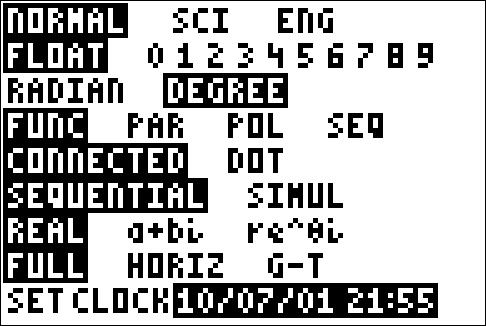
\includegraphics[width=2in]{./IntroTrigGraphics/UnitCircle01.jpg} &
\hspace{0.75in} 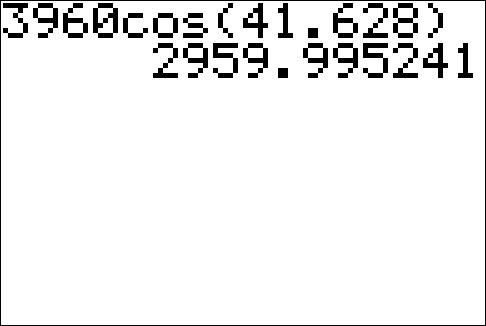
\includegraphics[width=2in]{./IntroTrigGraphics/UnitCircle02.jpg}  \\ 

\end{tabular} 

\end{center}

\vspace{-.35in} \qed

\end{enumerate}

\end{ex}

Theorem \ref{cosinesinecircle} gives us what we need to describe the position of an object traveling in a circular path of radius $r$ with constant angular velocity $\omega$.  Suppose that at time $t$, the object has swept out an angle measuring $\theta$ radians.  If we assume that the object is at the point $(r,0)$ when $t=0$, the angle $\theta$ is in standard position.  By definition, $\omega = \frac{\theta}{t}$ which we rewrite as  $\theta = \omega t$.  According to Theorem \ref{cosinesinecircle}, the location of the object $Q(x,y)$ on the circle is found using the equations  $x = r \cos(\theta) = r \cos(\omega t)$ and $y = r \sin(\theta) = r \sin(\omega t)$.  Hence, at time $t$, the object is at the point $(r \cos(\omega t), r \sin(\omega t))$.  We have just argued the following.


\smallskip

\colorbox{ResultColor}{\bbm
\begin{eqn} \label{equationsforcircularmotion} Suppose an object is traveling in a circular path of radius $r$ centered at the origin with constant angular velocity $\omega$.  If $t=0$ corresponds to the point $(r,0)$, then the $x$ and $y$ coordinates of the object are functions of $t$ and are given by $x =  r \cos(\omega t)$ and $y = r \sin(\omega t)$.  Here, $\omega > 0$ indicates a counter-clockwise direction and $\omega < 0$ indicates a clockwise direction.

\end{eqn}
\ebm}
\smallskip


\begin{center}

\hspace{.55in} \begin{mfpic}[15]{-5}{5}{-5}{5}
\axes
\tlabel(4.75,-0.5){\scriptsize $x$}
\tlabel(0.25,4.75){\scriptsize $y$}
\tlabel(2.1,-0.75){\scriptsize $1$}
\tlabel(0.25,2.1){\scriptsize $1$}
\tlabel(4.1,-0.75){\scriptsize $r$}
\tlabel(0.25,4.1){\scriptsize $r$}
\tlabel(2.35, 3.5){\small $Q\left(x,y\right) = (r \cos(\omega t), r \sin(\omega t))$}
\xmarks{-4 step 2 until 4}
\ymarks{-4 step 2 until 4}
\drawcolor[gray]{0.7}
\circle{(0,0),4}
\drawcolor[rgb]{0.33,0.33,0.33}
\arrow \polyline{(0,0), (2.5, 4.3301)}
\arrow \parafcn{5, 55, 5}{dir(t)}
\tlabel[cc](1.95, .5){\small $\theta = \omega t$}
\point[3pt]{(0,0),  (2, 3.4641)}
\penwd{1.5pt}
\arrow \parafcn{0, 60, 5}{4*dir(t)}
\end{mfpic} 

\hspace{-.7in} Equations for Circular Motion

\end{center}

\begin{ex}  Suppose we are in the situation of Example \ref{EarthRotationEx}.  Find the equations of motion of Lakeland Community College as the earth rotates.
\label{Lakelandrotates}

\smallskip

{\bf Solution.}  From Example \ref{EarthRotationEx}, we take $r = 2960$ miles and and $\omega = \frac{\pi}{12 \, \text{hours}}$.  Hence, the equations of motion are $x =  r \cos(\omega t) = 2960 \cos\left(\frac{\pi}{12} t\right)$ and  $y =  r \sin(\omega t) = 2960 \sin\left(\frac{\pi}{12} t\right)$, where $x$ and $y$ are measured in miles and $t$ is measured in hours. \qed

\end{ex}

In addition to circular motion, Theorem \ref{cosinesinecircle} is also the key to developing what is usually called `right triangle' trigonometry.\footnote{You may have been exposed to this in High School.}  As we shall see in the sections to come, many applications in trigonometry involve finding the measures of the angles in, and lengths of the sides of, right triangles.  Indeed, we made good use of some properties of right triangles to find the exact values of the cosine and sine of many of the angles in Example \ref{cosinesineviaunitcircle}, so the following development shouldn't be that much of a surprise.  Consider the generic right triangle below with corresponding acute angle $\theta$. The side with length $a$ is called the side of the triangle \emph{adjacent} to  $\theta$; the side with length $b$ is called the side of the triangle \emph{opposite} $\theta$; and the remaining side of length $c$ (the side opposite the right angle) is called the hypotenuse. We now imagine drawing this triangle in Quadrant I so that the angle $\theta$ is in standard position with the adjacent side to $\theta$ lying along the positive $x$-axis. 

\vspace{.1in}

\hspace{.5in} \begin{tabular}{m{2.5in}m{0.5in}m{2.5in}}

\begin{mfpic}[15]{-5}{5}{-5}{5}
\polyline{(-4.330,0), (4.330,0), (4.330,5), (-4.330,0)}
\arrow \reverse \arrow \shiftpath{(-4.330,0)} \parafcn{5, 25, 5}{3*dir(t)}
\tlabel(-1, 0.6){$\theta$}
\tlabel(0,-0.75){$a$}
\tlabel(4.75,2.25){$b$}
\tlabel(0,3){$c$}
\polyline{(3.93, 0), (3.93, 0.4), (4.33, 0.4)}
\end{mfpic}
&

&

\begin{mfpic}[15]{-5}{5}{-5}{5}
\axes
\tlabel(4.75,-0.5){\scriptsize $x$}
\tlabel(0.25,4.75){\scriptsize $y$}
\tlabel(4.1,-1){\scriptsize $c$}
\tlabel(0.25,4.1){\scriptsize $c$}
\xmarks{-4 step 4 until 4}
\ymarks{-4 step 4 until 4}
\tlabel(3.75,1.60){$P(a,b)$}
\drawcolor[gray]{0.7}
\circle{(0,0),4}
\drawcolor[rgb]{0.33,0.33,0.33}
\arrow \polyline{(0,0), (4.330,2.5)}
\arrow \parafcn{5, 25, 5}{1.5*dir(t)}
\tlabel(1.75, .25){\scriptsize $\theta$}
\point[3pt]{(0,0), (3.4641, 2)}
\polyline{(3.4641,2), (3.4641, 0)}
\polyline{(3.1641, 0), (3.1641, 0.3), (3.4641, 0.3)}
\end{mfpic} 

\end{tabular}

According to the Pythagorean Theorem, $a^2+b^2=c^2$, so that the point $P(a,b)$ lies on a circle of radius $c$.  Theorem \ref{cosinesinecircle} tells us that $\cos(\theta) = \frac{a}{c}$ and $\sin(\theta) = \frac{b}{c}$, so we have determined the cosine and sine of $\theta$ in terms of the lengths of the sides of the right triangle.  Thus we have the following theorem.
 
\smallskip

\colorbox{ResultColor}{\bbm

\begin{thm} \label{cosinesinetriangle}  Suppose $\theta$ is an acute angle residing in a right triangle.  If the length of the side adjacent to $\theta$ is $a$, the length of the side opposite $\theta$ is $b$, and the length of the hypotenuse is $c$, then $\cos(\theta) = \dfrac{a}{c}$ and $\sin(\theta) = \dfrac{b}{c}$.

\end{thm}

\ebm}

\smallskip

\begin{ex}  \label{righttriangleex} Find the measure of the missing angle and the lengths of the missing sides of:

\begin{center}

\begin{mfpic}[18]{-5}{5}{-5}{5}
\polyline{(-4.330,0), (4.330,0), (4.330,5), (-4.330,0)}
\arrow \reverse \arrow \shiftpath{(-4.330,0)} \parafcn{5, 25, 5}{3*dir(t)}
\tlabel(-1, 0.6){$30^{\circ}$}
\tlabel(0,-0.75){$7$}
\polyline{(3.93, 0), (3.93, 0.4), (4.33, 0.4)}
\end{mfpic}

\end{center}

{\bf Solution.}  The first and easiest task is to find the measure of the missing angle.  Since the sum of angles of a triangle is $180^{\circ}$, we know that the missing angle has measure $180^{\circ} - 30^{\circ} - 90^{\circ} = 60^{\circ}$.  We now proceed to find the lengths of the remaining two sides of the triangle.  Let $c$ denote the length of the hypotenuse of the triangle.  By Theorem \ref{cosinesinetriangle}, we have $\cos\left(30^{\circ}\right) = \frac{7}{c}$, or $c = \frac{7}{\cos\left(30^{\circ}\right)}$.  Since $\cos\left(30^{\circ}\right) = \frac{\sqrt{3}}{2}$, we have, after the usual fraction gymnastics, $c = \frac{14 \sqrt{3}}{3}$.  At this point, we have two ways to proceed to find the length of the side opposite the $30^{\circ}$ angle, which we'll denote $b$.  We know the length of the adjacent side is $7$ and the length of the hypotenuse is $\frac{14 \sqrt{3}}{3}$, so we could use the Pythagorean Theorem to find the missing side and solve  $(7)^2 + b^2 = \left( \frac{14 \sqrt{3}}{3} \right)^{2}$ for $b$.  Alternatively, we could use Theorem \ref{cosinesinetriangle}, namely that $\sin\left(30^{\circ}\right) = \frac{b}{c}$.  Choosing the latter, we find $b = c \sin\left(30^{\circ}\right) = \frac{14 \sqrt{3}}{3} \cdot \frac{1}{2} = \frac{7 \sqrt{3}}{3}$.  The triangle with all of its data is recorded below.

\begin{center}

\begin{mfpic}[18]{-5}{5}{-5}{5}
\polyline{(-4.330,0), (4.330,0), (4.330,5), (-4.330,0)}
\arrow \reverse \arrow \shiftpath{(-4.330,0)} \parafcn{5, 25, 5}{3*dir(t)}
\arrow \reverse \arrow \shiftpath{(4.330,5)}  \parafcn{215, 265, 5}{1.5*dir(t)}
\tlabel(-1, 0.6){$30^{\circ}$}
\tlabel(0,-0.75){$7$}
\tlabel(4.75,2.25){$b = \frac{7 \sqrt{3}}{3}$}
\tlabel(-2,3){$c = \frac{14 \sqrt{3}}{3}$}
\tlabel(2.75,2.9){$60^{\circ}$}
\polyline{(3.93, 0), (3.93, 0.4), (4.33, 0.4)}
\end{mfpic}

\end{center}

\vspace{-.45in} \qed

\end{ex}

\medskip

We close this section by noting that we can easily extend the functions cosine and sine to real numbers by identifying a real number $t$ with the angle $\theta = t$ radians.  Using this identification, we define $\cos(t) = \cos(\theta)$ and $\sin(t) = \sin(\theta)$. In practice this means expressions like $\cos(\pi)$ and $\sin(2)$ can be found by regarding the inputs as angles in radian measure or real numbers;  the choice is the reader's.  If we trace the identification of real numbers $t$ with angles $\theta$ in radian measure to its roots on page \pageref{wrappingfunction}, we can spell out this correspondence more precisely.  For each real number $t$, we associate an oriented arc $t$ units in length with initial point $(1,0)$ and endpoint $P(\cos(t), \sin(t))$.

\begin{tabular}{cc}

\begin{mfpic}[18]{-5}{5}{-4}{4.5}
\axes
\tlabel(4.75,-0.5){\scriptsize $x$}
\tlabel(0.25,4.25){\scriptsize $y$}
\tlabel(3.1,-0.75){\scriptsize $1$}
\tlabel(0.25,3.1){\scriptsize $1$}
\xmarks{-3 step 3 until 3}
\ymarks{-3 step 3 until 3}
\point[3pt]{(0,0)}
\drawcolor[gray]{0.7}
\circle{(0,0),3}
\drawcolor[rgb]{0.33,0.33,0.33}
\arrow \polyline{(0,0), (2.5, 4.3301)}
\arrow \reverse \arrow \polyline{(3,-4), (3,4.5)}
\polyline{(2.8,3.1416), (3.2,3.1416)}
\arrow \parafcn{5, 55, 5}{1.5*dir(t)}
\tlabel[cc](1.9, 1){$\theta = t$}
\penwd{1.5pt}
\arrow \polyline{(3,0), (3, 3.1416)}
\arrow \parafcn{0,60,5}{3*dir(t)}
\tlabel[cc](3.5,1.75){$t$}
\end{mfpic} 

&

\hspace{.3in}

\begin{mfpic}[18]{-5}{5}{-4}{4.5}
\axes
\tlabel(4.75,-0.5){\scriptsize $x$}
\tlabel(0.25,4.25){\scriptsize $y$}
\tlabel(3.1,-0.75){\scriptsize $1$}
\tlabel(0.25,3.1){\scriptsize $1$}
\xmarks{-3 step 3 until 3}
\ymarks{-3 step 3 until 3}
\arrow \polyline{(0,0), (2.5, 4.3301)}
\tlabel(2,2.6){$P(\cos(t), \sin(t))$}
\drawcolor[gray]{0.7}
\circle{(0,0),3}
\drawcolor[rgb]{0.33,0.33,0.33}
\arrow \parafcn{5, 55, 5}{1.5*dir(t)}
\tlabel[cc](1.9, 1){$\theta = t$}
\point[3pt]{(0,0), (1.5, 2.5981)}
\penwd{1.5pt}
\arrow \parafcn{0,60,5}{3*dir(t)}
\end{mfpic} 

\end{tabular}

In the same way we studied polynomial, rational, exponential, and logarithmic functions, we will study the trigonometric functions $f(t) = \cos(t)$ and $g(t) = \sin(t)$.  The first order of business is to find the domains and ranges of these functions.  Whether we think of identifying the real number $t$ with the angle $\theta = t$ radians, or think of wrapping an oriented arc around the Unit Circle to find coordinates on the Unit Circle, it should be clear that both the cosine and sine functions are defined for all real numbers $t$.  In other words, the domain  of $f(t) = \cos(t)$ and of $g(t) = \sin(t)$ is $(-\infty, \infty)$.  Since $\cos(t)$ and $\sin(t)$ represent $x$- and $y$-coordinates, respectively, of points on the Unit Circle, they both take on all of the values between $-1$ an $1$, inclusive.  In other words, the range of $f(t) = \cos(t)$ and of $g(t) = \sin(t)$ is the interval $[-1,1]$.  To summarize:

\smallskip

\colorbox{ResultColor}{\bbm

\begin{thm} \label{cosinesinefunctiondomainrange}  \textbf{Domain and Range of the Cosine and Sine Functions:} 

\vspace{.2in}

\begin{tabular}{ll}

\hspace{.3in} $\bullet \, $ The function $f(t) = \cos(t)$ & \hspace{.8in} $\bullet \, $ The function $g(t) = \sin(t)$ \\ [4pt]
\hspace{.5in} -- has domain $(-\infty, \infty)$ & \hspace{1in} -- has domain $(-\infty, \infty)$ \\ [4pt]
\hspace{.5in} -- has range $[-1,1]$ & \hspace{1in} -- has range $[-1,1]$ \\ [4pt]

\end{tabular}

\end{thm}

\ebm}

\smallskip
\phantomsection
\label{cosinesineequationsrealnumbers}

Suppose, as in the Exercises, we are asked to solve an equation such as $\sin(t) = -\frac{1}{2}$.  As we have already mentioned, the distinction between $t$ as a real number and as an angle $\theta = t$ radians is often blurred. Indeed, we solve $\sin(t) = -\frac{1}{2}$ in the exact same manner\footnote{Well, to be pedantic, we would be technically using `reference numbers' or `reference arcs' instead of `reference angles' -- but the idea is the same.} as we did in Example \ref{solveforangle} number \ref{sineisnegativehalf}.  Our solution is only cosmetically different in that the variable used is $t$ rather than $\theta$:  $t = \frac{7\pi}{6} + 2\pi k$ or  $t = \frac{11\pi}{6} + 2\pi k$ for integers, $k$.  We will study the cosine and sine functions in greater detail in Section \ref{TrigGraphs}.  Until then, keep in mind that any properties of cosine and sine developed in the following sections which regard them as functions of \textit{angles} in \textit{radian} measure apply equally well if the inputs are regarded as \textit{real numbers}.

\newpage

\subsection{Exercises}

In Exercises \ref{valuefirst} - \ref{valuelast}, find the exact value of the cosine and sine of the given angle.

\begin{multicols}{4}

\begin{enumerate}

\item $\theta = 0$ \vphantom{$\dfrac{\pi}{4}$} \label{valuefirst}
\item $\theta = \dfrac{\pi}{4}$
\item $\theta = \dfrac{\pi}{3}$
\item $\theta = \dfrac{\pi}{2}$

\setcounter{HW}{\value{enumi}}

\end{enumerate}

\end{multicols}

\begin{multicols}{4}

\begin{enumerate}

\setcounter{enumi}{\value{HW}}

\item $\theta = \dfrac{2\pi}{3}$
\item $\theta = \dfrac{3\pi}{4}$
\item $\theta = \pi$ \vphantom{$\dfrac{7\pi}{4}$}
\item $\theta = \dfrac{7\pi}{6}$

\setcounter{HW}{\value{enumi}}

\end{enumerate}

\end{multicols}

\begin{multicols}{4}

\begin{enumerate}

\setcounter{enumi}{\value{HW}}

\item $\theta = \dfrac{5\pi}{4}$
\item $\theta = \dfrac{4\pi}{3}$
\item $\theta = \dfrac{3\pi}{2}$
\item $\theta = \dfrac{5\pi}{3}$

\setcounter{HW}{\value{enumi}}

\end{enumerate}

\end{multicols}

\begin{multicols}{4}

\begin{enumerate}

\setcounter{enumi}{\value{HW}}

\item $\theta = \dfrac{7\pi}{4}$
\item $\theta = \dfrac{23\pi}{6}$
\item $\theta = -\dfrac{13\pi}{2}$
\item $\theta = -\dfrac{43\pi}{6}$

\setcounter{HW}{\value{enumi}}

\end{enumerate}

\end{multicols}

\begin{multicols}{4}

\begin{enumerate}

\setcounter{enumi}{\value{HW}}

\item $\theta = -\dfrac{3\pi}{4}$
\item $\theta = -\dfrac{\pi}{6}$ \vphantom{$\dfrac{7\pi}{4}$}
\item $\theta = \dfrac{10\pi}{3}$
\item $\theta = 117\pi$ \vphantom{$\dfrac{7\pi}{4}$} \label{valuelast}

\setcounter{HW}{\value{enumi}}

\end{enumerate}

\end{multicols}

In Exercises \ref{findthevaluefirst} - \ref{findthevaluelast}, use the results developed throughout the section to find the requested value.

\begin{enumerate}

\setcounter{enumi}{\value{HW}}

\item If $\sin(\theta) = -\dfrac{7}{25}$ with $\theta$ in Quadrant IV, what is $\cos(\theta)$? \label{findthevaluefirst}
\item If $\cos(\theta) = \dfrac{4}{9}$ with $\theta$ in Quadrant I, what is $\sin(\theta)$?
\item If $\sin(\theta) = \dfrac{5}{13}$ with $\theta$ in Quadrant II, what is $\cos(\theta)$?
\item If $\cos(\theta) = -\dfrac{2}{11}$ with $\theta$ in Quadrant III, what is $\sin(\theta)$?
\item If $\sin(\theta) = -\dfrac{2}{3}$ with $\theta$ in Quadrant III, what is $\cos(\theta)$?
\item If $\cos(\theta) = \dfrac{28}{53}$ with $\theta$ in Quadrant IV, what is $\sin(\theta)$?
\item  If $\sin(\theta) = \dfrac{2\sqrt{5}}{5}$ and $\dfrac{\pi}{2} < \theta < \pi$, what is $\cos(\theta)$?
\item  If $\cos(\theta) = \dfrac{\sqrt{10}}{10}$ and $2\pi < \theta < \dfrac{5\pi}{2}$, what is $\sin(\theta)$?
\item  If $\sin(\theta) = -0.42$ and $\pi < \theta < \dfrac{3\pi}{2}$, what is  $\cos(\theta)$?
\item  If $\cos(\theta) = -0.98$ and $\dfrac{\pi}{2} < \theta < \pi$, what is $\sin(\theta)$? \label{findthevaluelast}

\setcounter{HW}{\value{enumi}}

\end{enumerate}

\pagebreak

In Exercises \ref{solveforanglefirst} - \ref{solveforanglelast}, find all of the angles which satisfy the given equation.

\begin{multicols}{3}

\begin{enumerate}

\setcounter{enumi}{\value{HW}}

\item $\sin(\theta) = \dfrac{1}{2}$ \vphantom{$\dfrac{2}{2}$} \label{solveforanglefirst}
\item $\cos(\theta) = -\dfrac{\sqrt{3}}{2}$
\item $\sin(\theta) = 0$ \vphantom{$\dfrac{2}{2}$}

\setcounter{HW}{\value{enumi}}

\end{enumerate}

\end{multicols}

\begin{multicols}{3}

\begin{enumerate}

\setcounter{enumi}{\value{HW}}

\item $\cos(\theta) = \dfrac{\sqrt{2}}{2}$
\item $\sin(\theta) = \dfrac{\sqrt{3}}{2}$
\item $\cos(\theta) = -1$ \vphantom{$\dfrac{\sqrt{2}}{2}$}

\setcounter{HW}{\value{enumi}}

\end{enumerate}

\end{multicols}

\begin{multicols}{3}

\begin{enumerate}

\setcounter{enumi}{\value{HW}}

\item  $\sin(\theta) = -1$ \vphantom{$\dfrac{\sqrt{2}}{2}$}
\item  $\cos(\theta) = \dfrac{\sqrt{3}}{2}$
\item  $\cos(\theta) = -1.001$ \vphantom{$\dfrac{\sqrt{2}}{2}$} \label{solveforanglelast}

\setcounter{HW}{\value{enumi}}

\end{enumerate}

\end{multicols}

In Exercises \ref{solvefortfirst} - \ref{solvefortlast}, solve the equation for $t$.  (See the comments following Theorem \ref{cosinesinefunctiondomainrange}.)

\begin{multicols}{3}

\begin{enumerate}

\setcounter{enumi}{\value{HW}}

\item $\cos(t) = 0$ \vphantom{$\dfrac{\sqrt{2}}{2}$} \label{solvefortfirst}
\item $\sin(t) = -\dfrac{\sqrt{2}}{2}$
\item $\cos(t) = 3$ \vphantom{$\dfrac{\sqrt{2}}{2}$}

\setcounter{HW}{\value{enumi}}

\end{enumerate}

\end{multicols}

\begin{multicols}{3}

\begin{enumerate}

\setcounter{enumi}{\value{HW}}

\item $\sin(t) = -\dfrac{1}{2}$
\item $\cos(t) = \dfrac{1}{2}$
\item $\sin(t) = -2$ \vphantom{$\dfrac{1}{2}$}

\setcounter{HW}{\value{enumi}}

\end{enumerate}

\end{multicols}

\begin{multicols}{3}

\begin{enumerate}

\setcounter{enumi}{\value{HW}}

\item $\cos(t) = 1$ \vphantom{$\dfrac{\sqrt{2}}{2}$}
\item $\sin(t) = 1$ \vphantom{$\dfrac{\sqrt{2}}{2}$}
\item $\cos(t) = -\dfrac{\sqrt{2}}{2}$ \label{solvefortlast}

\setcounter{HW}{\value{enumi}}

\end{enumerate}

\end{multicols}

In Exercises \ref{calculatorfirst} - \ref{calculatorlast}, use your calculator to approximate the given value to three decimal places.  Make sure your calculator is in the proper angle measurement mode!

\begin{multicols}{3}

\begin{enumerate}

\setcounter{enumi}{\value{HW}}

\item $\sin(78.95^{\circ})$ \label{calculatorfirst}
\item $\cos(-2.01)$
\item $\sin(392.994)$

\setcounter{HW}{\value{enumi}}

\end{enumerate}

\end{multicols}

\begin{multicols}{3}

\begin{enumerate}

\setcounter{enumi}{\value{HW}}

\item $\cos(207^{\circ})$
\item $\sin\left( \pi^{\circ} \right)$
\item $\cos(e)$ \label{calculatorlast} 

\setcounter{HW}{\value{enumi}}

\end{enumerate}

\end{multicols}

In Exercises \ref{firsttriangle} - \ref{lasttriangle}, find the measurement of the missing angle and the lengths of the missing sides.  (See Example \ref{righttriangleex})

\begin{multicols}{2}

\begin{enumerate}

\setcounter{enumi}{\value{HW}}

\item Find $\theta$, $b$, and $c$. \label{firsttriangle}

 \begin{mfpic}[15]{-5}{5}{-5}{5}
\polyline{(-4.330,0), (4.330,0), (4.330,5), (-4.330,0)}
\arrow \reverse \arrow \shiftpath{(-4.330,0)} \parafcn{5, 25, 5}{3*dir(t)}
\arrow \reverse \arrow \shiftpath{(4.330,5)}  \parafcn{215, 265, 5}{1.5*dir(t)}
\tlabel(-1, 0.6){$30^{\circ}$}
\tlabel(0,-0.75){$1$}
\tlabel(4.75,2.25){$b$}
\tlabel(-0.5,3){$c$}
\tlabel(3,3){$\theta$}
\polyline{(3.93, 0), (3.93, 0.4), (4.33, 0.4)}
\end{mfpic}

\item  Find $\theta$, $a$, and $c$.

\begin{mfpic}[18]{-5}{5}{-5}{5}
\polyline{(-2.5, 0), (2.5,0), (-2.5,5), (-2.5,0)}
\arrow \reverse \arrow \shiftpath{(2.5,0)} \parafcn{140, 175, 5}{1.5*dir(t)}
\arrow \reverse \arrow \shiftpath{(-2.5,5)}  \parafcn{275, 310, 5}{1.5*dir(t)}
\tlabel(-2, 2.75){$45^{\circ}$}
\tlabel(-0.5,-0.75){$3$}
\tlabel(-3.25,2.25){$a$}
\tlabel(0,3){$c$}
\tlabel(0.5,0.5){$\theta$}
\polyline{(-2.5, 0.4), (-2.1, 0.4), (-2.1, 0)}
\end{mfpic}

\setcounter{HW}{\value{enumi}}

\end{enumerate}

\end{multicols}

\pagebreak

\begin{multicols}{2}

\begin{enumerate}

\setcounter{enumi}{\value{HW}}

\item  Find $\alpha$, $a$, and $b$.

\begin{mfpic}[18]{-1}{5}{-1}{7}
\polyline{(0,0), (0,6.709), (4.357, 6.709), (0,0)}
\arrow \reverse \arrow \parafcn{60, 87, 5}{1.75*dir(t)}
\arrow \reverse \arrow \shiftpath{(4.357,6.709)}  \parafcn{185, 232, 5}{1.5*dir(t)}
\tlabel(0.25, 2){$33^{\circ}$}
\tlabel(3,3){$8$}
\tlabel(2,7){$b$}
\tlabel(-0.75,4){$a$}
\tlabel(2.25,5.75){$\alpha$}
\polyline{(0,6.304), (0.4, 6.304),  (0.4, 6.704)}
\end{mfpic}

\item Find $\beta$, $a$, and $c$. \label{lasttriangle}

\begin{mfpic}[18]{-6}{1}{-1}{9}
\polyline{(0,0), (0,6), (-5.402, 6), (0,0)}
\arrow \reverse \arrow \parafcn{95, 127, 5}{1.75*dir(t)}
\arrow \reverse \arrow \shiftpath{(-5.402,6)}  \parafcn{317, 355, 5}{1.5*dir(t)}
\tlabel(-3.75, 5){$48^{\circ}$}
\tlabel(0.5,3){$6$}
\tlabel(-2.6,6.25){$a$}
\tlabel(-3.25,2.5){$c$}
\tlabel(-1,2){$\beta$}
\polyline{(0,5.6), (-0.4, 5.6),  (-0.4, 6)}
\end{mfpic} 

\setcounter{HW}{\value{enumi}}

\end{enumerate}

\end{multicols}

In Exercises \ref{missingsidefirst} - \ref{missingsidelast}, assume that $\theta$ is an acute angle in a right triangle and use Theorem \ref{cosinesinetriangle} to find the requested side.

\begin{enumerate}

\setcounter{enumi}{\value{HW}}

\item If $\theta = 12^{\circ}$ and the side adjacent to $\theta$ has length 4, how long is the hypotenuse? \label{missingsidefirst}
\item If $\theta = 78.123^{\circ}$ and the hypotenuse has length 5280, how long is the side adjacent to $\theta$?
\item If $\theta = 59^{\circ}$ and the side opposite $\theta$ has length 117.42, how long is the hypotenuse?
\item If $\theta = 5^{\circ}$ and the hypotenuse has length 10, how long is the side opposite $\theta$?
\item If $\theta = 5^{\circ}$ and the hypotenuse has length 10, how long is the side adjacent to $\theta$?
\item If $\theta = 37.5^{\circ}$ and the side opposite $\theta$ has length 306, how long is the side adjacent to $\theta$? \label{missingsidelast}

\setcounter{HW}{\value{enumi}}

\end{enumerate}

In Exercises \ref{pointsfirst} - \ref{pointslast}, let $\theta$ be the angle in standard position whose terminal side contains the given point then compute $\cos(\theta)$ and $\sin(\theta)$.

\begin{multicols}{4}

\begin{enumerate}

\setcounter{enumi}{\value{HW}}

\item $P(-7, 24)$ \label{pointsfirst} 
\item $Q(3, 4)$
\item $R(5, -9)$
\item $T(-2, -11)$ \label{pointslast}

\setcounter{HW}{\value{enumi}}

\end{enumerate}

\end{multicols}

In Exercises \ref{motionfirst} - \ref{motionlast}, find the equations of motion for the given scenario.  Assume that the center of the motion is the origin, the motion is counter-clockwise and that $t = 0$ corresponds to a position along the positive $x$-axis.  (See Equation \ref{equationsforcircularmotion} and Example \ref{EarthRotationEx}.)

\begin{enumerate}

\setcounter{enumi}{\value{HW}}

\item  \label{motionfirst} A point on the edge of the spinning yo-yo in Exercise \ref{spinningyoyo} from Section \ref{Angles}. 

Recall: The diameter of the yo-yo is 2.25 inches and it spins at 4500 revolutions per minute.

\item  The yo-yo in exercise \ref{yoyotrick} from Section \ref{Angles}.

Recall: The radius of the circle is 28 inches and it completes one revolution in 3 seconds.

\item A point on the edge of the hard drive in Exercise \ref{harddrive} from Section \ref{Angles}.

Recall:  The diameter of the hard disk is 2.5 inches and it spins at 7200 revolutions per minute.

\item  \label{motionlast} A passenger on the Big Wheel in Exercise \ref{giantwheelmotion} from Section \ref{Angles}.

Recall: The diameter is 128 feet and completes 2 revolutions in 2 minutes, 7 seconds.

\setcounter{HW}{\value{enumi}}

\end{enumerate}

\begin{enumerate}

\setcounter{enumi}{\value{HW}}

\item Consider the numbers:  $0$, $1$, $2$, $3$, $4$.  Take the square root of each of these numbers, then divide each by $2$. The resulting numbers should look hauntingly familiar. (See the values in the table on \pageref{CosineSineFacts}.) 

\item Let $\alpha$ and $\beta$ be the two acute angles of a right triangle.  (Thus $\alpha$ and $\beta$ are complementary angles.)  Show that $\sin(\alpha) = \cos(\beta)$ and $\sin(\beta) = \cos(\alpha)$.  The fact that co-functions of complementary angles are equal in this case is not an accident and a more general result will be given in Section \ref{Identities}.
\label{cofunctionforeshadowing}

\item  In the scenario of Equation \ref{equationsforcircularmotion}, we assumed that at $t=0$, the object was at the point $(r,0)$.  If this is not the case,  we can adjust the equations of motion by introducing a `time delay.'   If $t_{0} > 0$ is the first time the object passes through the point $(r,0)$, show, with the help of your classmates, the equations of motion are $x = r \cos(\omega (t - t_{0}))$ and $y = r \sin(\omega (t-t_{0}))$.

\end{enumerate}

\newpage

\subsection{Answers}

\begin{multicols}{2}

\begin{enumerate}

\item $\cos(0) = 1$, $\; \sin(0) = 0$ \vphantom{$\dfrac{\sqrt{2}}{2}$}

\item $\cos \left(\dfrac{\pi}{4} \right) = \dfrac{\sqrt{2}}{2}$, $\; \sin \left(\dfrac{\pi}{4} \right) = \dfrac{\sqrt{2}}{2}$

\setcounter{HW}{\value{enumi}}

\end{enumerate}

\end{multicols}

\begin{multicols}{2}

\begin{enumerate}

\setcounter{enumi}{\value{HW}}

\item $\cos \left(\dfrac{\pi}{3}\right) = \dfrac{1}{2}$, $\; \sin \left(\dfrac{\pi}{3}\right) = \dfrac{\sqrt{3}}{2}$

\item $\cos \left(\dfrac{\pi}{2}\right) = 0$, $\; \sin \left(\dfrac{\pi}{2}\right) = 1$ \vphantom{$\dfrac{\sqrt{2}}{2}$}

\setcounter{HW}{\value{enumi}}

\end{enumerate}

\end{multicols}

\begin{multicols}{2}

\begin{enumerate}

\setcounter{enumi}{\value{HW}}

\item $\cos\left(\dfrac{2\pi}{3}\right) = -\dfrac{1}{2}$, $\; \sin \left(\dfrac{2\pi}{3}\right) = \dfrac{\sqrt{3}}{2}$

\item $\cos \left(\dfrac{3\pi}{4} \right) = -\dfrac{\sqrt{2}}{2}$, $\; \sin \left(\dfrac{3\pi}{4} \right) = \dfrac{\sqrt{2}}{2}$

\setcounter{HW}{\value{enumi}}

\end{enumerate}

\end{multicols}

\begin{multicols}{2}

\begin{enumerate}

\setcounter{enumi}{\value{HW}}

\item $\cos(\pi) = -1$, $\; \sin(\pi) = 0$ \vphantom{$\dfrac{\sqrt{3}}{2}$}

\item $\cos\left(\dfrac{7\pi}{6}\right) = -\dfrac{\sqrt{3}}{2}$, $\; \sin\left(\dfrac{7\pi}{6}\right) = -\dfrac{1}{2}$

\setcounter{HW}{\value{enumi}}

\end{enumerate}

\end{multicols}

\begin{multicols}{2}

\begin{enumerate}

\setcounter{enumi}{\value{HW}}

\item $\cos \left(\dfrac{5\pi}{4} \right) = -\dfrac{\sqrt{2}}{2}$, $\; \sin \left(\dfrac{5\pi}{4} \right) = -\dfrac{\sqrt{2}}{2}$

\item $\cos\left(\dfrac{4\pi}{3}\right) = -\dfrac{1}{2}$, $\; \sin \left(\dfrac{4\pi}{3}\right) = -\dfrac{\sqrt{3}}{2}$

\setcounter{HW}{\value{enumi}}

\end{enumerate}

\end{multicols}

\begin{multicols}{2}

\begin{enumerate}

\setcounter{enumi}{\value{HW}}

\item $\cos \left(\dfrac{3\pi}{2}\right) = 0$, $\; \sin \left(\dfrac{3\pi}{2}\right) = -1$

\item $\cos\left(\dfrac{5\pi}{3}\right) = \dfrac{1}{2}$, $\; \sin \left(\dfrac{5\pi}{3}\right) = -\dfrac{\sqrt{3}}{2}$

\setcounter{HW}{\value{enumi}}

\end{enumerate}

\end{multicols}

\begin{multicols}{2}

\begin{enumerate}

\setcounter{enumi}{\value{HW}}

\item $\cos \left(\dfrac{7\pi}{4} \right) = \dfrac{\sqrt{2}}{2}$, $\; \sin \left(\dfrac{7\pi}{4} \right) = -\dfrac{\sqrt{2}}{2}$

\item $\cos\left(\dfrac{23\pi}{6}\right) = \dfrac{\sqrt{3}}{2}$, $\; \sin\left(\dfrac{23\pi}{6}\right) = -\dfrac{1}{2}$

\setcounter{HW}{\value{enumi}}

\end{enumerate}

\end{multicols}

\begin{multicols}{2}

\begin{enumerate}

\setcounter{enumi}{\value{HW}}

\item $\cos \left(-\dfrac{13\pi}{2}\right) = 0$, $\; \sin \left(-\dfrac{13\pi}{2}\right) = -1$ \vphantom{$\dfrac{\sqrt{3}}{2}$}

\item $\cos\left(-\dfrac{43\pi}{6}\right) = -\dfrac{\sqrt{3}}{2}$, $\; \sin\left(-\dfrac{43\pi}{6}\right) = \dfrac{1}{2}$

\setcounter{HW}{\value{enumi}}

\end{enumerate}

\end{multicols}

\begin{multicols}{2}

\begin{enumerate}

\setcounter{enumi}{\value{HW}}

\item $\cos \left(-\dfrac{3\pi}{4} \right) = -\dfrac{\sqrt{2}}{2}$, $\; \sin \left(-\dfrac{3\pi}{4} \right) = -\dfrac{\sqrt{2}}{2}$

\item $\cos\left(-\dfrac{\pi}{6}\right) = \dfrac{\sqrt{3}}{2}$, $\; \sin\left(-\dfrac{\pi}{6}\right) = -\dfrac{1}{2}$

\setcounter{HW}{\value{enumi}}

\end{enumerate}

\end{multicols}

\begin{multicols}{2}

\begin{enumerate}

\setcounter{enumi}{\value{HW}}

\item $\cos\left(\dfrac{10\pi}{3}\right) = -\dfrac{1}{2}$, $\; \sin \left(\dfrac{10\pi}{3}\right) = -\dfrac{\sqrt{3}}{2}$

\item $\cos(117\pi) = -1$, $\; \sin(117\pi) = 0$ \vphantom{$\dfrac{\sqrt{3}}{2}$}

\setcounter{HW}{\value{enumi}}

\end{enumerate}

\end{multicols}

\begin{enumerate}

\setcounter{enumi}{\value{HW}}

\item If $\sin(\theta) = -\dfrac{7}{25}$ with $\theta$ in Quadrant IV, then $\cos(\theta) = \dfrac{24}{25}$.
\item If $\cos(\theta) = \dfrac{4}{9}$ with $\theta$ in Quadrant I, then $\sin(\theta) = \dfrac{\sqrt{65}}{9}$.
\item If $\sin(\theta) = \dfrac{5}{13}$ with $\theta$ in Quadrant II, then $\cos(\theta) = -\dfrac{12}{13}$.
\item If $\cos(\theta) = -\dfrac{2}{11}$ with $\theta$ in Quadrant III, then $\sin(\theta) = -\dfrac{\sqrt{117}}{11}$.
\item If $\sin(\theta) = -\dfrac{2}{3}$ with $\theta$ in Quadrant III, then $\cos(\theta) = -\dfrac{\sqrt{5}}{3}$.
\item If $\cos(\theta) = \dfrac{28}{53}$ with $\theta$ in Quadrant IV, then $\sin(\theta) = -\dfrac{45}{53}$.
\item  If $\sin(\theta) = \dfrac{2\sqrt{5}}{5}$ and $\dfrac{\pi}{2} < \theta < \pi$, then $\cos(\theta) = -\dfrac{\sqrt{5}}{5}$.
\item  If $\cos(\theta) = \dfrac{\sqrt{10}}{10}$ and $2\pi < \theta < \dfrac{5\pi}{2}$, then $\sin(\theta)  = \dfrac{3 \sqrt{10}}{10}$.
\item  If $\sin(\theta) = -0.42$ and $\pi < \theta < \dfrac{3\pi}{2}$, then $\cos(\theta) = -\sqrt{0.8236} \approx -0.9075$.
\item  If $\cos(\theta) = -0.98$ and $\dfrac{\pi}{2} < \theta < \pi$, then $\sin(\theta) = \sqrt{0.0396} \approx 0.1990$.

\setcounter{HW}{\value{enumi}}

\end{enumerate}

\begin{enumerate}

\setcounter{enumi}{\value{HW}}

\item $\sin(\theta) = \dfrac{1}{2}$ when $\theta = \dfrac{\pi}{6} + 2\pi k$ or $\theta = \dfrac{5\pi}{6} + 2\pi k$ for any integer $k$.
\item $\cos(\theta) = -\dfrac{\sqrt{3}}{2}$ when $\theta = \dfrac{5\pi}{6} + 2\pi k$ or $\theta = \dfrac{7\pi}{6} + 2\pi k$ for any integer $k$.
\item $\sin(\theta) = 0$ when $\theta = \pi k$ for any integer $k$.
\item $\cos(\theta) = \dfrac{\sqrt{2}}{2}$ when $\theta = \dfrac{\pi}{4} + 2\pi k$ or $\theta = \dfrac{7\pi}{4} + 2\pi k$ for any integer $k$.
\item $\sin(\theta) = \dfrac{\sqrt{3}}{2}$ when $\theta = \dfrac{\pi}{3} + 2\pi k$ or $\theta = \dfrac{2\pi}{3} + 2\pi k$ for any integer $k$.
\item $\cos(\theta) = -1$ when $\theta = (2k + 1)\pi$ for any integer $k$.
\item  $\sin(\theta) = -1$ when $\theta = \dfrac{3\pi}{2} + 2\pi k$ for any integer $k$.
\item  $\cos(\theta) = \dfrac{\sqrt{3}}{2}$ when $\theta = \dfrac{\pi}{6} + 2\pi k$ or  $\theta = \dfrac{11\pi}{6} + 2\pi k$ for any integer $k$.
%\item  $\sin(\theta) = \dfrac{\sqrt{2}}{2}$ when $\theta = \dfrac{\pi}{4} + 2\pi k$ or  $\theta = \dfrac{3\pi}{4} + 2\pi k$ for any integer $k$.
\item  $\cos(\theta) = -1.001$ never happens

\setcounter{HW}{\value{enumi}}

\end{enumerate}

\begin{enumerate}

\setcounter{enumi}{\value{HW}}

\item $\cos(t) = 0$ when $t = \dfrac{\pi}{2} + \pi k$ for any integer $k$.
\item $\sin(t) = -\dfrac{\sqrt{2}}{2}$ when $t = \dfrac{5\pi}{4} + 2\pi k$ or $t = \dfrac{7\pi}{4} + 2\pi k$ for any integer $k$.
\item $\cos(t) = 3$ never happens.  
\item $\sin(t) = -\dfrac{1}{2}$ when $t = \dfrac{7\pi}{6} + 2\pi k$ or $t = \dfrac{11\pi}{6} + 2\pi k$ for any integer $k$.
\item $\cos(t) = \dfrac{1}{2}$ when $t = \dfrac{\pi}{3} + 2\pi k$ or $t = \dfrac{5\pi}{3} + 2\pi k$ for any integer $k$.
\item $\sin(t) = -2$ never happens
\item $\cos(t) = 1$ when $t = 2\pi k$ for any integer $k$.
\item $\sin(t) = 1$ when $t = \dfrac{\pi}{2} + 2\pi k$ for any integer $k$.
\item $\cos(t) = -\dfrac{\sqrt{2}}{2}$ when $t = \dfrac{3\pi}{4} + 2\pi k$ or $t = \dfrac{5\pi}{4} + 2\pi k$ for any integer $k$.
%\item  $\sin(t) = -\dfrac{\sqrt{3}}{2}$ when $t = \dfrac{4\pi}{3} + 2\pi k$ or  $t = \dfrac{5\pi}{3} + 2\pi k$ for any integer $k$.

\setcounter{HW}{\value{enumi}}

\end{enumerate}

\begin{multicols}{3}

\begin{enumerate}

\setcounter{enumi}{\value{HW}}

\item $\sin(78.95^{\circ}) \approx 0.981$
\item $\cos(-2.01) \approx -0.425$
\item $\sin(392.994) \approx -0.291$

\setcounter{HW}{\value{enumi}}

\end{enumerate}

\end{multicols}

\begin{multicols}{3}

\begin{enumerate}

\setcounter{enumi}{\value{HW}}

\item $\cos(207^{\circ}) \approx -0.891$
\item $\sin\left( \pi^{\circ} \right) \approx 0.055$
\item $\cos(e) \approx -0.912$

\setcounter{HW}{\value{enumi}}

\end{enumerate}

\end{multicols}

\begin{enumerate}

\setcounter{enumi}{\value{HW}}

\item $\theta = 60^{\circ}$, $b = \dfrac{ \sqrt{3}}{3}$, $c=\dfrac{2 \sqrt{3}}{3}$

\item  $\theta = 45^{\circ}$, $a = 3$, $c = 3\sqrt{2}$

\item  $\alpha = 57^{\circ}$, $a = 8 \cos(33^{\circ}) \approx 6.709$, $b = 8 \sin(33^{\circ}) \approx 4.357$

\item  $\beta = 42^{\circ}$, $c = \dfrac{6}{\sin(48^{\circ})} \approx 8.074$, $a = \sqrt{c^2 - 6^2} \approx 5.402$

\setcounter{HW}{\value{enumi}}

\end{enumerate}


\begin{enumerate}

\setcounter{enumi}{\value{HW}}

\item The hypotenuse has length $\dfrac{4}{\cos(12^{\circ})}\approx 4.089$.
\item The side adjacent to $\theta$ has length $5280\cos(78.123^{\circ}) \approx 1086.68$.
\item The hypotenuse has length $\dfrac{117.42}{\sin(59^{\circ})}\approx 136.99$.
\item The side opposite $\theta$ has length $10\sin(5^{\circ}) \approx 0.872$.
\item The side adjacent to $\theta$ has length $10\cos(5^{\circ}) \approx 9.962$.
\item The hypotenuse has length $c = \dfrac{306}{\sin(37.5^{\circ})}\approx 502.660$, so the side adjacent to $\theta$ has length  $\sqrt{c^2 - 306^{2}} \approx 398.797$.

\setcounter{HW}{\value{enumi}}

\end{enumerate}

\begin{enumerate}

\setcounter{enumi}{\value{HW}}

\item $\cos(\theta) = -\dfrac{7}{25}, \; \sin(\theta) = \dfrac{24}{25}$

\item $\cos(\theta) = \dfrac{3}{5}, \; \sin(\theta) = \dfrac{4}{5}$

\item $\cos(\theta) = \dfrac{5\sqrt{106}}{106}, \; \sin(\theta) = -\dfrac{9\sqrt{106}}{106}$

\item $\cos(\theta) = -\dfrac{2\sqrt{5}}{25}, \; \sin(\theta) = -\dfrac{11\sqrt{5}}{25}$

\setcounter{HW}{\value{enumi}}

\end{enumerate}

\begin{enumerate}

\setcounter{enumi}{\value{HW}}

\item   $r = 1.125$ inches, $\omega = 9000 \pi \, \frac{\text{radians}}{\text{minute}}$,  $x = 1.125 \cos(9000 \pi \, t)$, $y = 1.125 \sin(9000 \pi \, t)$.  Here $x$ and $y$ are measured in inches and $t$ is measured in minutes.

\item   $r = 28$ inches, $\omega = \frac{2\pi}{3} \, \frac{\text{radians}}{\text{second}}$,  $x = 28 \cos\left(\frac{2\pi}{3} \, t \right)$, $y = 28 \sin\left(\frac{2\pi}{3} \, t \right)$.  Here $x$ and $y$ are measured in inches and $t$ is measured in seconds.

\item $r = 1.25$ inches, $\omega = 14400 \pi \, \frac{\text{radians}}{\text{minute}}$,  $x = 1.25 \cos(14400 \pi \, t)$, $y = 1.25 \sin(14400 \pi \, t)$.  Here $x$ and $y$ are measured in inches and $t$ is measured in minutes.

\item  $r = 64$ feet, $\omega = \frac{4\pi}{127} \, \frac{\text{radians}}{\text{second}}$,  $x = 64 \cos\left(\frac{4\pi}{127} \, t \right)$, $y = 64 \sin\left(\frac{4\pi}{127} \, t \right)$.  Here $x$ and $y$ are measured in feet and $t$ is measured in seconds

\end{enumerate}


\closegraphsfile